% !TEX program = pdflatex
\documentclass[aspectratio=169, 10pt]{beamer}

\usetheme{metropolis}

% ---------------------------------------------------------------------------
% COLOR & FONT TWEAKS  (matches nn_lecture.tex palette)
% ---------------------------------------------------------------------------
\definecolor{ColumbiaBlue}{HTML}{185494}
\definecolor{AccentOrange}{HTML}{E8792B}
\definecolor{LightGray}{HTML}{F5F5F5}
\definecolor{CodeBg}{HTML}{F0F0F0}
\definecolor{AlertRed}{HTML}{C0392B}
\definecolor{GoodGreen}{HTML}{27AE60}
\definecolor{AccentGreen}{HTML}{27AE60}

\setbeamercolor{frametitle}{bg=ColumbiaBlue, fg=white}
\setbeamercolor{progress bar}{fg=AccentOrange}
\setbeamercolor{alerted text}{fg=AccentOrange}
\setbeamercolor{block title}{bg=ColumbiaBlue!15, fg=ColumbiaBlue}
\setbeamercolor{block body}{bg=ColumbiaBlue!5}
\setbeamercolor{block title alerted}{bg=AlertRed!15, fg=AlertRed}
\setbeamercolor{block body alerted}{bg=AlertRed!5}
\setbeamercolor{block title example}{bg=GoodGreen!15, fg=GoodGreen!80!black}
\setbeamercolor{block body example}{bg=GoodGreen!5}

\metroset{
  sectionpage=progressbar,
  subsectionpage=none,
  numbering=fraction,
  progressbar=frametitle,
  block=fill,
}

% ---------------------------------------------------------------------------
% PACKAGES
% ---------------------------------------------------------------------------
\usepackage{amsmath, amssymb, bm}
\usepackage{booktabs}
\usepackage{graphicx}
\usepackage{listings}
\usepackage{tikz}
\usetikzlibrary{arrows.meta, positioning, fit, calc, decorations.pathreplacing}
\usepackage{pifont}
\usepackage{xcolor}
\usepackage{hyperref}
\usepackage{appendixnumberbeamer}
\usepackage{array}

% ---------------------------------------------------------------------------
% CUSTOM COMMANDS  (matches nn_lecture.tex)
% ---------------------------------------------------------------------------
\newcommand{\notebookcallout}[2]{%
  \vspace{4pt}%
  \noindent\begin{tikzpicture}
    \node[
      fill=AccentOrange!10,
      draw=AccentOrange,
      rounded corners=4pt,
      inner sep=5pt,
      font=\scriptsize,
      text width=0.90\textwidth,
      align=left,
    ] {%
      {\color{AccentOrange}\ding{118}\;\textbf{Notebook \S#1}} --- #2%
    };
  \end{tikzpicture}%
}

\newcommand{\keyword}[1]{\textcolor{ColumbiaBlue}{\textbf{#1}}}
\newcommand{\bad}[1]{\textcolor{AlertRed}{#1}}
\newcommand{\good}[1]{\textcolor{GoodGreen!80!black}{#1}}

% ---------------------------------------------------------------------------
% TITLE
% ---------------------------------------------------------------------------
\title{Large Language Models:\\From N-Grams to the Attention Revolution}
\subtitle{BINF 4002 --- Machine Learning for Health}
\author{Matthew McDermott}
\institute{Department of Biomedical Informatics, Columbia University}
\date{}

% ===========================================================================
\begin{document}
% ===========================================================================

\maketitle

% ---------------------------------------------------------------------------
\begin{frame}{Roadmap}

\begin{columns}[T]
\column{0.48\textwidth}
\begin{enumerate}
  \item \textbf{The Paradox} --- Searle's Chinese Room
  \item \textbf{Language Modeling} --- what the problem really is
  \item \textbf{Why It's Hard} --- sparsity, n-grams, combinatorics
\end{enumerate}

\column{0.48\textwidth}
\begin{enumerate}\setcounter{enumi}{3}
  \item \textbf{The Transformer} --- how attention solves it
  \item \textbf{The LLM Ecosystem} --- how to actually use them
  \item \textbf{Open Challenges} --- what remains unsolved
\end{enumerate}
\end{columns}

\vspace{10pt}
\begin{center}
\small Experiments and walkthroughs in the companion notebook.\\
\textcolor{AccentOrange}{\ding{118}} \textbf{Notebook:} \texttt{llm\_lecture\_notebook.ipynb}
\end{center}

\end{frame}

% ===========================================================================
\section{The Paradox}
% ===========================================================================

% ---------------------------------------------------------------------------
\begin{frame}{Today's Paradox: The Chinese Room}

\begin{columns}[T]
\column{0.54\textwidth}

\begin{block}{Searle (1980): A thought experiment}
\vspace{2pt}
Imagine you are locked in a room.
\begin{itemize}
  \item<2-> You receive slips of paper with \textbf{Chinese symbols}.
  \item<3-> A \textbf{rulebook} (in English) tells you exactly which symbols to write back.
  \item<4-> You pass responses through a slot.
  \item<5-> To anyone outside, you appear to \textbf{understand Chinese}.
\end{itemize}
\end{block}

\onslide<6->{
\vspace{6pt}
\begin{alertblock}{The question}
You follow rules. You produce fluent output.\\
But do you \emph{understand} anything?
\end{alertblock}
}

\column{0.43\textwidth}
\onslide<2->{
\vspace{6pt}
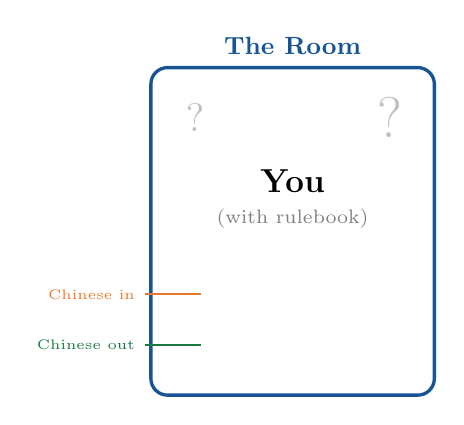
\begin{tikzpicture}[scale=0.80]
  \draw[very thick, ColumbiaBlue, rounded corners=6pt] (0,0) rectangle (4.5,5.2);
  \node[ColumbiaBlue, font=\small\bfseries] at (2.25,5.55) {The Room};
  \node[font=\large\bfseries] at (2.25,3.4) {You};
  \node[font=\scriptsize, gray] at (2.25,2.8) {(with rulebook)};
  \draw[thick, AccentOrange] (-0.1,1.6) -- (0.8,1.6);
  \node[left, font=\tiny, AccentOrange] at (-0.1,1.6) {Chinese in};
  \draw[thick, GoodGreen!70!black] (-0.1,0.8) -- (0.8,0.8);
  \node[left, font=\tiny, GoodGreen!70!black] at (-0.1,0.8) {Chinese out};
  \node[font=\huge, gray!50] at (3.8,4.4) {?};
  \node[font=\Large, gray!50] at (0.7,4.4) {?};
\end{tikzpicture}
}

\end{columns}
\end{frame}

% ---------------------------------------------------------------------------
\begin{frame}{Why Philosophers Cared --- A Lot}

\begin{columns}[T]
\column{0.50\textwidth}

\onslide<1->{
\begin{block}{The target: Strong AI}
\vspace{2pt}
\small The dominant view before 1980: \keyword{functionalism}. If a system produces the right outputs from the right inputs, it \emph{has} a mind. Behavior is sufficient for understanding.
\vspace{14pt}
\end{block}
}

\vspace{3pt}

\onslide<2->{
\begin{alertblock}{Searle's challenge}
\vspace{2pt}
\small The Chinese Room shows you can produce \textbf{all the right outputs} with \textbf{zero understanding}. Syntax alone cannot generate semantics.
\vspace{2pt}
\end{alertblock}
}

\column{0.47\textwidth}

\onslide<3->{
\begin{block}{Why the field split: replies}
\vspace{2pt}
\scriptsize
\begin{itemize}\itemsep3pt
  \item \textbf{Systems reply}: the whole \emph{system} understands, not just you. \\\textit{Searle}: memorize the full rulebook --- do you understand now?
  \item \textbf{Robot reply}: ground the system in a body and sensors.\\\textit{Searle}: still symbol manipulation, just with richer inputs.
  \item \textbf{Brain simulator}: simulate actual neurons.\\\textit{Searle}: simulating water doesn't make you wet.
  \item \textbf{Functionalists}: behavior \emph{is} mind. None of these replies concede the point.
\end{itemize}
\end{block}
}

\end{columns}

\vspace{4pt}
\onslide<4->{
\begin{exampleblock}{The verdict}
\small One of the most cited papers in philosophy of mind. No consensus. The debate is \textbf{still open} --- and now suddenly practical.
\end{exampleblock}
}

\end{frame}

% ===========================================================================
\section{Language Modeling}
% ===========================================================================

% ---------------------------------------------------------------------------
% Slide 1: The big question
\begin{frame}{}

\begin{center}
\vspace{1.5cm}
{\LARGE Suppose a system could finish any sentence\\[10pt]
the way a \keyword{knowledgeable person} would.}

\vspace{1.5cm}

\onslide<2->{
{\large What could you do with that?}
}
\end{center}

\end{frame}

% ---------------------------------------------------------------------------
% Slide 2: The prompt
\begin{frame}{What Text Comes Next?}

\begin{center}
\vspace{0.6cm}
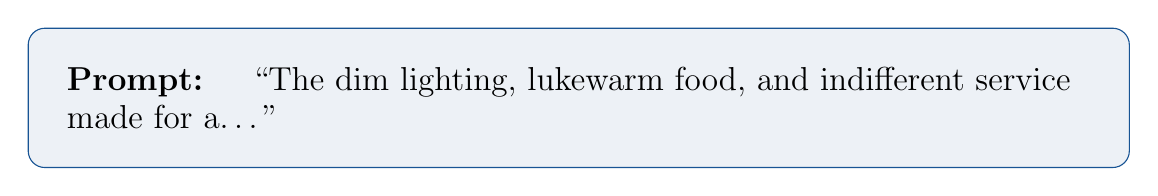
\begin{tikzpicture}
  \node[draw=ColumbiaBlue, fill=ColumbiaBlue!8, rounded corners=6pt,
        inner sep=14pt, text width=13cm, font=\large] {
    \textbf{Prompt:} \quad ``The dim lighting, lukewarm food, and indifferent service made for a\dots''
  };
\end{tikzpicture}

\vspace{1.0cm}

\begin{columns}[T]
\column{0.46\textwidth}
\onslide<2->{
\begin{exampleblock}{\large Completion A}
\vspace{4pt}
``\dots\ a \textbf{delightful} evening. The chef clearly cares about every dish.''
\vspace{4pt}
\end{exampleblock}
}

\column{0.46\textwidth}
\onslide<3->{
\begin{alertblock}{\large Completion B}
\vspace{4pt}
``\dots\ The mitochondria is the powerhouse of the cell.''
\vspace{4pt}
\end{alertblock}
}
\end{columns}
\end{center}

\end{frame}

% ---------------------------------------------------------------------------
% Slide 3: Round 2 -- harder
\begin{frame}{Now a Harder Question}

\begin{center}
\vspace{0.4cm}
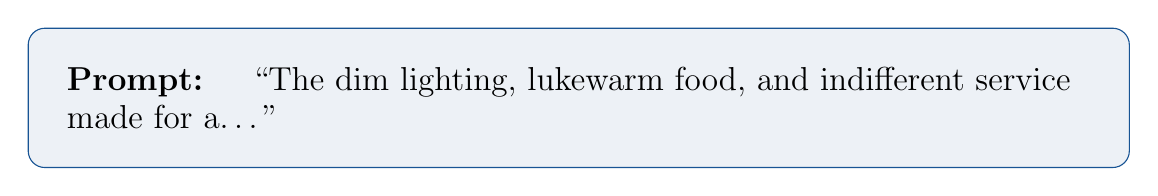
\begin{tikzpicture}
  \node[draw=ColumbiaBlue, fill=ColumbiaBlue!8, rounded corners=6pt,
        inner sep=14pt, text width=13cm, font=\large] {
    \textbf{Prompt:} \quad ``The dim lighting, lukewarm food, and indifferent service made for a\dots''
  };
\end{tikzpicture}

\vspace{0.8cm}

\begin{columns}[T]
\column{0.46\textwidth}
\begin{exampleblock}{\large Completion A}
\vspace{4pt}
``\dots\ a \textbf{delightful} evening. The chef clearly cares about every dish.''
\vspace{4pt}
\end{exampleblock}

\column{0.46\textwidth}
\onslide<2->{
\begin{alertblock}{\large Completion B}
\vspace{4pt}
``\dots\ a \textbf{disappointing} evening. I would not return.''
\vspace{4pt}
\end{alertblock}
}
\end{columns}

\end{center}

\end{frame}

% ---------------------------------------------------------------------------
% Slide 4: The key insight
\begin{frame}{The Key Insight}

\begin{center}
\vspace{0.4cm}
{\large The prompt described \bad{dim lighting}, \bad{lukewarm food}, and \bad{indifferent service}.}

\vspace{0.8cm}
\onslide<2->{
{\large A model that truly understands language\\[6pt]
must assign \bad{``disappointing''} far higher probability than \good{``delightful''}\\[6pt]
given that context.}
}

\vspace{0.8cm}
\onslide<3->{
\begin{block}{}
\centering
\large If it can do \emph{this}, it can classify sentiment, answer questions,\\
reason clinically --- \textbf{almost any task is a completion task.}
\end{block}
}
\end{center}

\end{frame}

% ---------------------------------------------------------------------------
% Slide 5: Probability formulation
\begin{frame}{Language Modeling as a Probability Problem}

\only<1>{
\vspace{8pt}
By the \textbf{chain rule of probability}, any sequence probability factors into next-word predictions:
\[
  P(w_1, \ldots, w_T)
  = \prod_{t=1}^{T} P(w_t \mid w_1, \ldots, w_{t-1})
\]
\vspace{8pt}
}

\onslide<2->{
\begin{exampleblock}{The key reduction}
To model any sequence, \textbf{all we need} is to predict the next word given everything before it.

\vspace{6pt}
\begin{center}
\textbf{(1)} Score a sequence \qquad \textbf{(2)} Predict the next word \qquad \textbf{(3)} Generate new text
\end{center}
\end{exampleblock}
}

\vspace{10pt}

\onslide<3->{
From our review prompt, a trained model should assign:
\[
P(\text{``disappointing''} \mid \text{context}) \;\gg\; P(\text{``delightful''} \mid \text{context})
\]
The model must learn --- from data --- to assign high probability to contextually appropriate words.
}

\end{frame}

% ===========================================================================
\section{From Na\"{i}ve Lookup to Transformers}
% ===========================================================================

% ---------------------------------------------------------------------------
\begin{frame}{A Na\"{i}ve Approach: Just Look It Up}

\onslide<1->{
\textbf{Simplest possible idea:} given a context, search a large corpus for \emph{exact matches} and see what word came next. No model --- just a lookup table.
}

\vspace{6pt}

\begin{columns}[T]
\column{0.50\textwidth}
\onslide<2->{
\begin{block}{Shorter queries work fine}
\textit{``the''} --- billions of matches.\\
\textit{``the film''} --- millions of matches.\\
\textit{``thoroughly disappointing''} --- many matches.
\end{block}
}
\onslide<3->{
\begin{alertblock}{Longer queries: zero matches}
\vspace{2pt}
\textit{``The dim lighting, lukewarm food, and indifferent service made for a thoroughly''}\\[4pt]
Even with $10^{12}$ tokens of text (CommonCrawl scale), this context appears \textbf{exactly zero times} in any corpus.
\end{alertblock}
}

\column{0.46\textwidth}
\onslide<4->{
\begin{block}{Why does this happen?}
The space of possible contexts is \textbf{combinatorially enormous}. Even a modest sentence is effectively unique. We cannot rely on having seen it before.
\end{block}
}
\onslide<4->{
\notebookcallout{1}{Empirically verify this on a real corpus. Measure exact-match counts as context length increases.}
}
\end{columns}

\end{frame}

% ---------------------------------------------------------------------------
\begin{frame}{§1 Notebook: Match Counts Drop to Zero Fast}

\begin{center}
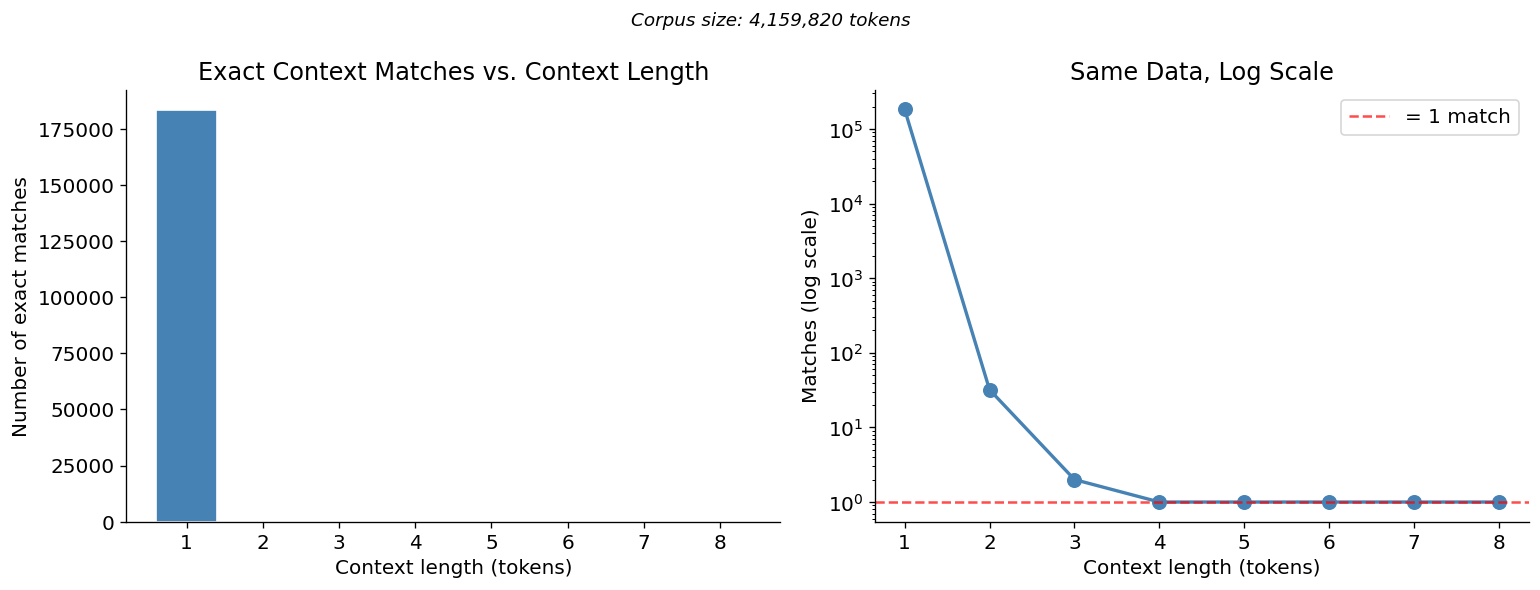
\includegraphics[width=0.92\textwidth]{figures/nb_context_matches.png}
\end{center}

\vspace{2pt}
\begin{center}
\textit{PubMed corpus (4.2M tokens). Even 2-word queries are vanishingly rare; 4-word queries functionally never repeat.}
\end{center}

\end{frame}

% ---------------------------------------------------------------------------
\begin{frame}{N-gram Models: Use Only the Last $n$ Words}

\onslide<1->{
\textbf{Idea:} if the full context never matches, use only the \emph{last} $n{-}1$ words (Markov assumption):
\[
  P(w_t \mid w_1, \ldots, w_{t-1}) \;\approx\; P(w_t \mid w_{t-n+1}, \ldots, w_{t-1})
\]
Estimate from counts in a corpus. Simple, fast, and surprisingly effective for small $n$.
}

\vspace{4pt}

\begin{columns}[T]
\column{0.48\textwidth}

\onslide<2->{
\begin{exampleblock}{Unigram ($n=1$): $P(w_t)$}
\vspace{2pt}
\textit{``the patient of sessions sirna developed injection in gray prescription phosphenes ivu\dots''}
\end{exampleblock}
}

\onslide<3->{
\begin{exampleblock}{Bigram ($n=2$): $P(w_t \mid w_{t-1})$}
\vspace{2pt}
\textit{``the patient resulting in the results from additional dose pantoprazole on production of patients with respect to\dots''}
\end{exampleblock}
}

\column{0.48\textwidth}

\onslide<4->{
\begin{exampleblock}{Trigram ($n=3$): $P(w_t \mid w_{t-2}, w_{t-1})$}
\vspace{2pt}
\textit{``the patient underwent an integrated and linked to the existing drg as indirect support for the determination of malignancy\dots''}
\end{exampleblock}
}

\onslide<5->{
\begin{exampleblock}{5-gram ($n=5$)}
\vspace{2pt}
\textit{``the patient was adherent to treatment he had decreased level of consciousness she underwent whole body positron emission tomography\dots''}
\end{exampleblock}
}

\end{columns}

\onslide<5->{
\vspace{2pt}
\notebookcallout{2}{Build n-gram models for $n \in \{1,2,3,5\}$. Generate and compare text. See how quality evolves.}
}

\end{frame}

% ---------------------------------------------------------------------------
\begin{frame}{Why We Can't Just Use Larger $n$}

\onslide<1->{
\begin{center}
\large\textbf{Discussion question:}\\[10pt]
\end{center}
}

\onslide<1->{
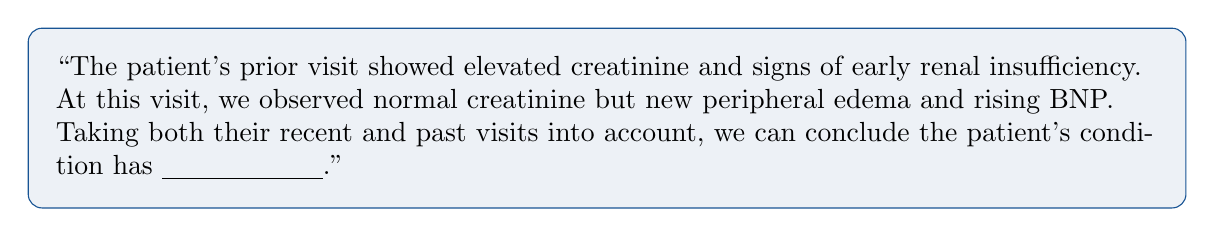
\begin{tikzpicture}
  \node[draw=ColumbiaBlue, fill=ColumbiaBlue!8, rounded corners=5pt,
        inner sep=10pt, text width=14cm, font=\normalsize] {
    ``The patient's prior visit showed elevated creatinine and signs of early renal insufficiency.
    At this visit, we observed normal creatinine but new peripheral edema and rising BNP.
    Taking both their recent and past visits into account, we can conclude the patient's condition
    has \underline{\phantom{xxxxxxxxxxx}}.''
  };
\end{tikzpicture}
}

\vspace{8pt}
\onslide<2->{
\begin{center}
What fills the blank? \quad What \emph{evidence} does it depend on?
\end{center}
}

\end{frame}

% ---------------------------------------------------------------------------
\begin{frame}{Long-Range Dependencies}

\begin{columns}[T]
\column{0.50\textwidth}
\onslide<1->{
\begin{block}{The answer requires the full context}
\vspace{4pt}
\textit{``\dots\ the patient's condition has \textbf{evolved} / \textbf{worsened} / \textbf{shifted}.''}

\vspace{6pt}
The right completion depends on \emph{both} visits: improving creatinine from the prior visit \emph{and} new edema/BNP from this visit. Neither alone is sufficient.
\end{block}
}

\column{0.47\textwidth}
\onslide<2->{
\begin{alertblock}{What n-gram models predict at the blank}
\vspace{4pt}
\textbf{2-gram} top-5: \texttt{the, in, by, for, using}\\[3pt]
\textbf{3-gram}: no matching context found\\
\textbf{5-gram}: no matching context found\\[4pt]
The key word ``patient'' is more than 5 tokens back --- simply \textbf{out of window} at any practical $n$.
\end{alertblock}
}
\end{columns}

\vspace{6pt}
\onslide<3->{
\begin{exampleblock}{The catch}
Increasing $n$ would help --- but the parameter space grows so fast that large $n$ is physically unreachable. We're stuck.
\end{exampleblock}
}

\onslide<3->{
\notebookcallout{2}{Test this: what does your n-gram model predict for the blank?}
}

\end{frame}

% ---------------------------------------------------------------------------
\begin{frame}{The Combinatorial Abyss: Why Context Scales Are Unreachable}

\vspace{4pt}

\begin{center}
\begin{tabular}{@{}r r l@{}}
\toprule
\textbf{Context length} & \textbf{Possible contexts ($V^n$)} & \textbf{Comparison} \\
\midrule
\visible<1->{1 token}     & \visible<1->{$5 \times 10^{4}$}        & \visible<1->{Trivial} \\
\visible<2->{2 tokens}    & \visible<2->{$2.5 \times 10^{9}$}      & \visible<2->{$>$ world population} \\
\visible<3->{4 tokens}    & \visible<3->{$6.3 \times 10^{18}$}     & \visible<3->{$\approx$ grains of sand on Earth's beaches} \\
\visible<4->{6 tokens}    & \visible<4->{$1.6 \times 10^{28}$}     & \visible<4->{$\gg$ stars in the observable universe} \\
\visible<5->{10 tokens}   & \visible<5->{$\approx 10^{47}$}        & \visible<5->{$\gg$ atoms in the Milky Way} \\
\visible<6->{20 tokens}   & \visible<6->{$\approx 10^{94}$}        & \visible<6->{$\gg$ atoms in the observable universe} \\
\visible<7->{128K tokens} & \visible<7->{$\approx 10^{600{,}000}$} & \visible<7->{\bad{Incomprehensibly beyond physical reality}} \\
\bottomrule
\end{tabular}
\end{center}

\vspace{3pt}
\onslide<8->{
\begin{alertblock}{The conclusion}
We cannot enumerate all contexts. We \emph{cannot} use n-grams at the scales modern LLMs operate at. We need a model that \textbf{generalizes without memorizing} --- and one that can handle arbitrarily long context.
\end{alertblock}
}

\end{frame}

% ===========================================================================
\section{The Transformer}
% ===========================================================================

% ---------------------------------------------------------------------------
\begin{frame}{What We Need From a Language Model}

\onslide<1->{We need a learned function from context to next-word probabilities. What properties must it have?}

\vspace{10pt}

\begin{enumerate}
  \item<2-> \textbf{Variable-length input} --- sentences are not all the same length.
  \item<3-> \textbf{Long-range dependencies} --- context from far away must be reachable.
  \item<4-> \textbf{Valid probability output} --- a proper distribution over the vocabulary at each step.
  \item<5-> \textbf{Order sensitivity} --- \textit{``dog bites man''} $\neq$ \textit{``man bites dog''}.
  \item<6-> \textbf{Scalable training} --- must work with trillions of tokens and billions of parameters.
\end{enumerate}

\end{frame}

% ---------------------------------------------------------------------------
% NEW SLIDE A: High-level prediction diagram
\begin{frame}{A Language Model: The Big Picture}

\begin{center}
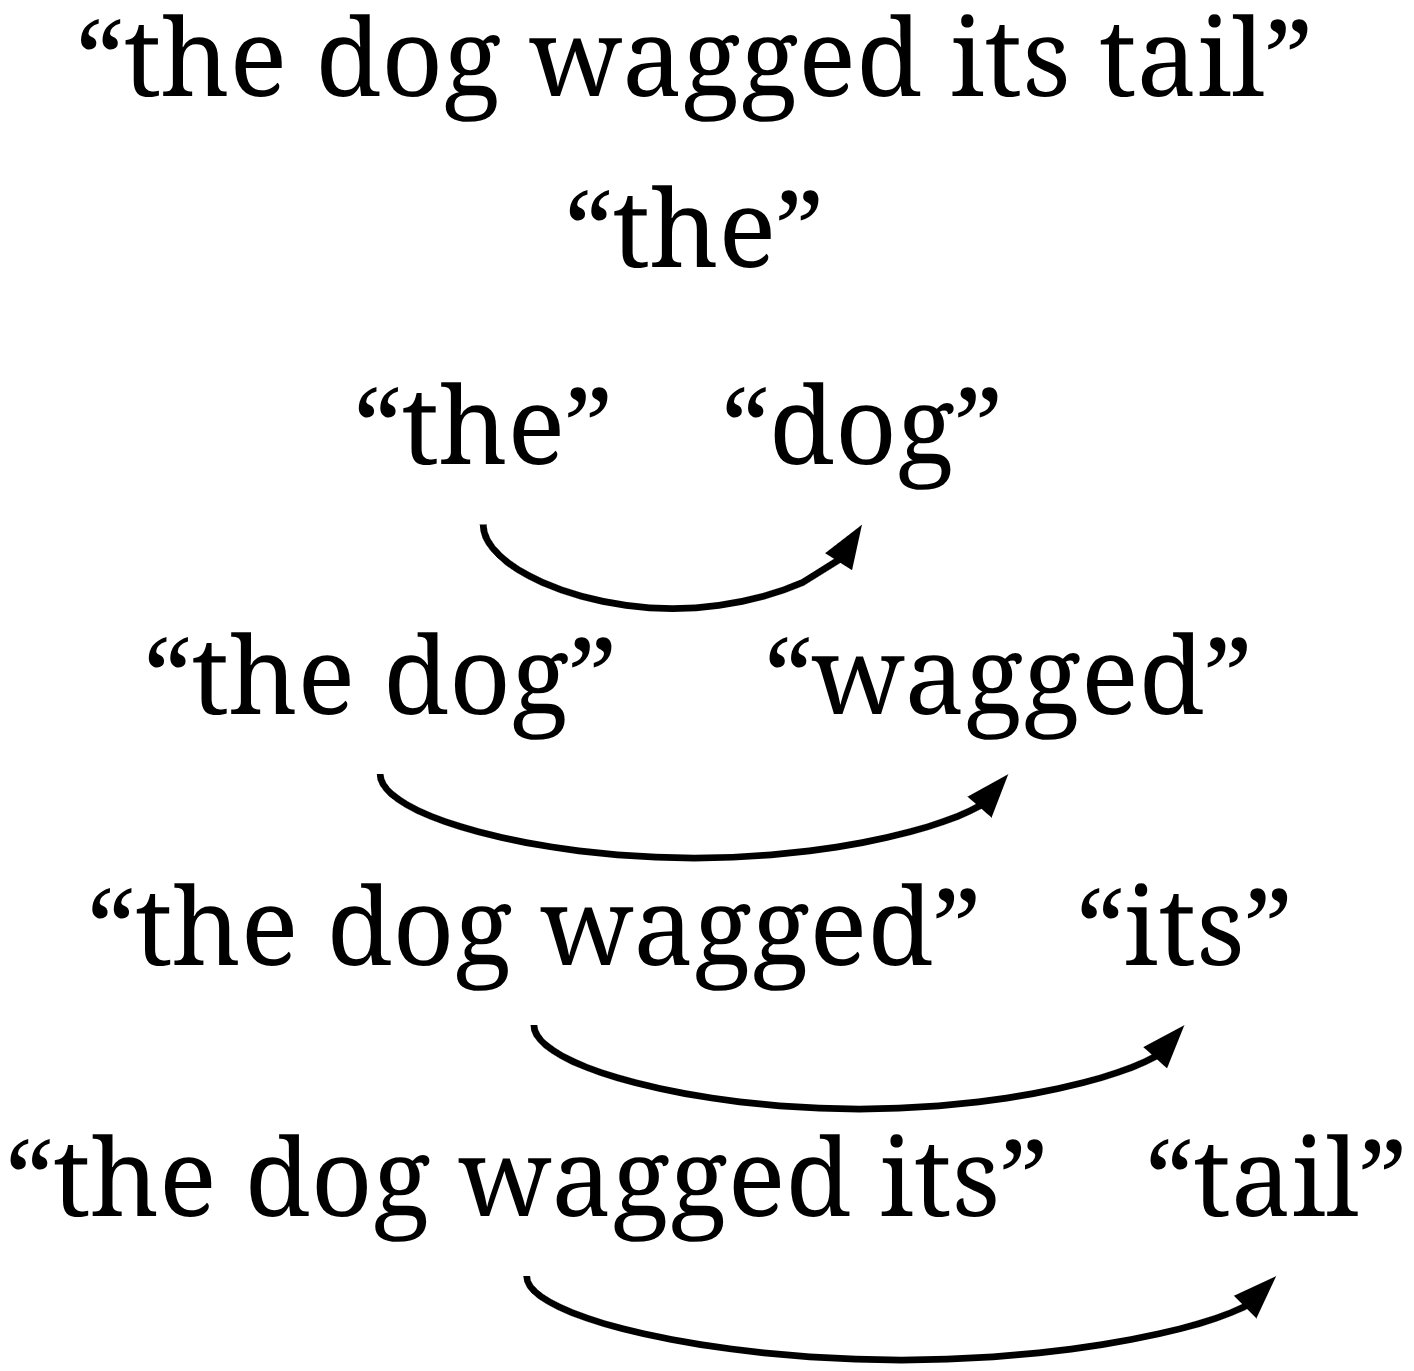
\includegraphics[height=0.72\textheight, keepaspectratio]{figures/LM_prediction.png}
\end{center}

\onslide<2->{
\begin{center}
\small Each prefix predicts the next word. We append it and repeat --- generation is just next-token prediction, applied autoregressively.
\end{center}
}

\end{frame}

% ---------------------------------------------------------------------------
% NEW SLIDE B: Word embeddings
\begin{frame}{Step 1: Words $\to$ Vectors (Embeddings)}

\onslide<1->{
\begin{alertblock}{The problem}
Neural networks operate on real-valued vectors. Words are discrete symbols. We need a bridge.
\end{alertblock}
}

\vspace{8pt}

\begin{columns}[T]
\column{0.50\textwidth}
\onslide<2->{
\begin{block}{The embedding lookup}
Every token in the vocabulary gets a trainable vector $\mathbf{e} \in \mathbb{R}^d$ (typically $d = 512$--$4096$).

\vspace{6pt}
\begin{center}
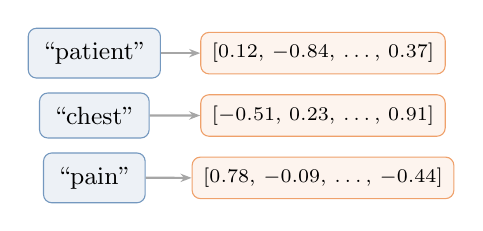
\begin{tikzpicture}[scale=0.88,
  tok/.style={draw=ColumbiaBlue!60, fill=ColumbiaBlue!8, rounded corners=3pt, inner sep=5pt, font=\small},
  vec/.style={draw=AccentOrange!70, fill=AccentOrange!8, rounded corners=3pt, inner sep=4pt, font=\scriptsize},
  arr/.style={-{Stealth[length=4pt]}, thick, gray!70},
]
\node[tok] (w1) at (0,0)   {``patient''};
\node[tok] (w2) at (0,-0.9) {``chest''};
\node[tok] (w3) at (0,-1.8) {``pain''};
\node[vec] (v1) at (3.3, 0)    {$[0.12,\,-0.84,\,\ldots,\,0.37]$};
\node[vec] (v2) at (3.3, -0.9)  {$[-0.51,\,0.23,\,\ldots,\,0.91]$};
\node[vec] (v3) at (3.3, -1.8)  {$[0.78,\,-0.09,\,\ldots,\,-0.44]$};
\draw[arr] (w1) -- (v1);
\draw[arr] (w2) -- (v2);
\draw[arr] (w3) -- (v3);
\end{tikzpicture}
\end{center}
\end{block}
}

\column{0.47\textwidth}
\onslide<3->{
\begin{block}{What embeddings learn}
Directions in embedding space encode meaning:
\begin{itemize}
  \item Similar words cluster together
  \item Analogies become vector arithmetic
  \item Medical synonyms get similar vectors after training on clinical text
\end{itemize}
\end{block}

}
\end{columns}

\end{frame}

% ---------------------------------------------------------------------------
% NEW SLIDE C: Decoder-only transformer structure
\begin{frame}{The Decoder-Only Transformer (GPT Family)}

\begin{center}
    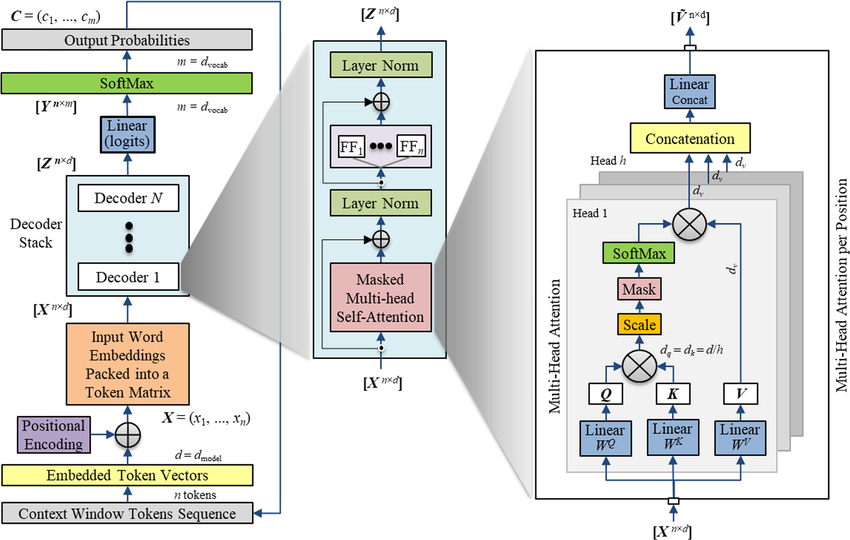
\includegraphics[width=0.7\linewidth]{figures/Overview-of-the-GPT-architecture.png}
\end{center}

% \begin{columns}[T]
% \column{0.38\textwidth}
% \begin{center}
% \begin{tikzpicture}[
%   box/.style={draw=ColumbiaBlue, fill=ColumbiaBlue!10, rounded corners=4pt,
%               text width=3.6cm, align=center, inner sep=6pt, font=\small},
%   attn/.style={draw=AccentOrange, fill=AccentOrange!10, rounded corners=4pt,
%                text width=3.6cm, align=center, inner sep=6pt, font=\small},
%   ff/.style={draw=GoodGreen!70!black, fill=GoodGreen!8, rounded corners=4pt,
%              text width=3.6cm, align=center, inner sep=6pt, font=\small},
%   outbox/.style={draw=ColumbiaBlue!60, fill=ColumbiaBlue!5, rounded corners=4pt,
%               text width=3.6cm, align=center, inner sep=6pt, font=\small},
%   arr/.style={-{Stealth[length=5pt]}, thick, gray!70},
%   brace/.style={decorate, decoration={brace, amplitude=5pt}, thick, ColumbiaBlue!50},
% ]
% % Input
% \node[box] (emb) at (0, 0)    {Token + Positional\\Embeddings};
% % Attention block
% \node[attn] (attn) at (0,-1.5) {Masked\\Self-Attention\\+ Add \& Norm};
% % FF block
% \node[ff]   (ff)   at (0,-3.0) {Feed-Forward\\+ Add \& Norm};
% % Output head
% \node[outbox]  (lm)   at (0,-4.5) {Linear + Softmax};
% % Output label
% \node[font=\small, GoodGreen!80!black] (prob) at (0,-5.4) {$P(\text{next token})$};

% \draw[arr] (emb)  -- (attn);
% \draw[arr] (attn) -- (ff);
% \draw[arr] (ff)   -- (lm);
% \draw[arr] (lm)   -- (prob);

% % Brace for N× repetition
% \draw[brace] (2.1,-1.1) -- (2.1,-3.4)
%   node[midway, right=6pt, font=\small, ColumbiaBlue] {$\times N$};
% \end{tikzpicture}
% \end{center}

% \column{0.58\textwidth}
% \vspace{4pt}
% \onslide<2->{
% \begin{block}{The core loop}
% \begin{itemize}
%   \item Each \textbf{block} applies masked attention then a feed-forward layer, both wrapped with residual connections
%   \item Blocks are stacked $N$ times (GPT-3: $N=96$)
%   \item \textbf{Causal mask}: token $t$ can only attend to positions $\leq t$ --- no peeking at future tokens
% \end{itemize}
% \end{block}
% }

% \vspace{6pt}
% \onslide<3->{
% \begin{block}{Key asymmetry}
% \textbf{Attention} mixes information \emph{across all tokens} simultaneously --- it is a sequence-level operation.\\[4pt]
% \textbf{Feed-forward} is applied \emph{independently to each token} --- same weights, one token at a time.
% \end{block}
% }
% \end{columns}

\end{frame}

\begin{frame}{Each Transformer Layer}

\begin{center}
    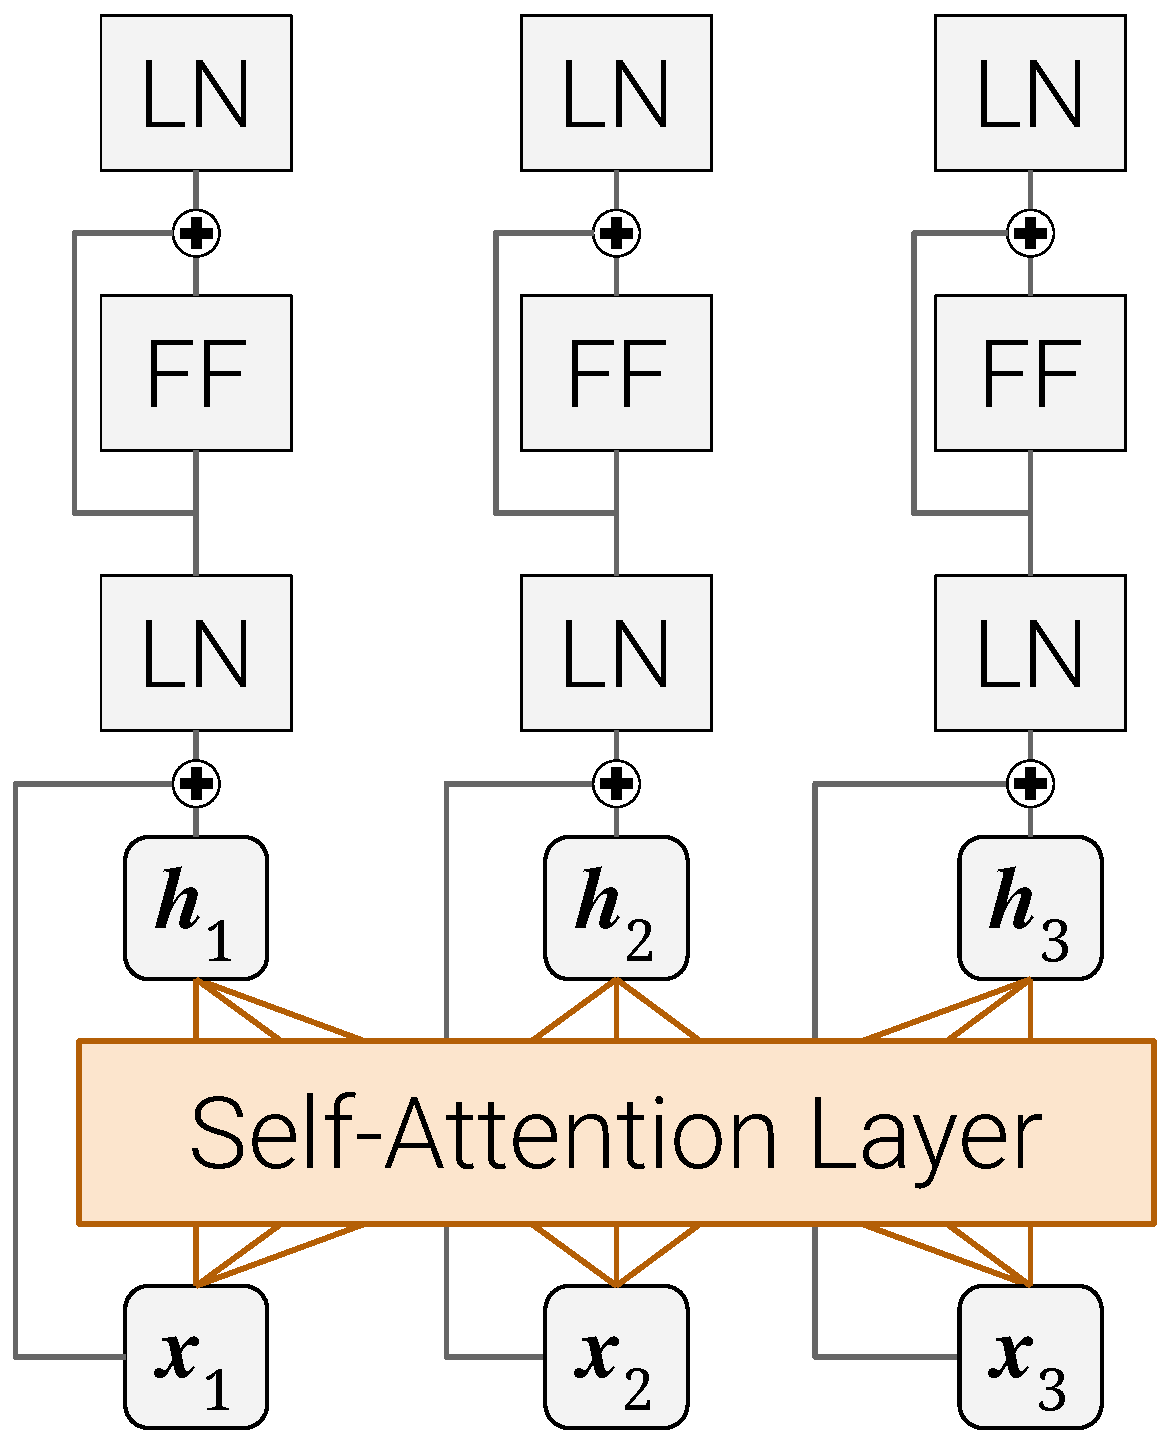
\includegraphics[width=0.4\linewidth]{figures/Transformer Layer Block.pdf}
\end{center}

\end{frame}

% ---------------------------------------------------------------------------
% \begin{frame}{The Transformer Architecture}

% \begin{columns}[T]
% \column{0.50\textwidth}

% \begin{center}
% 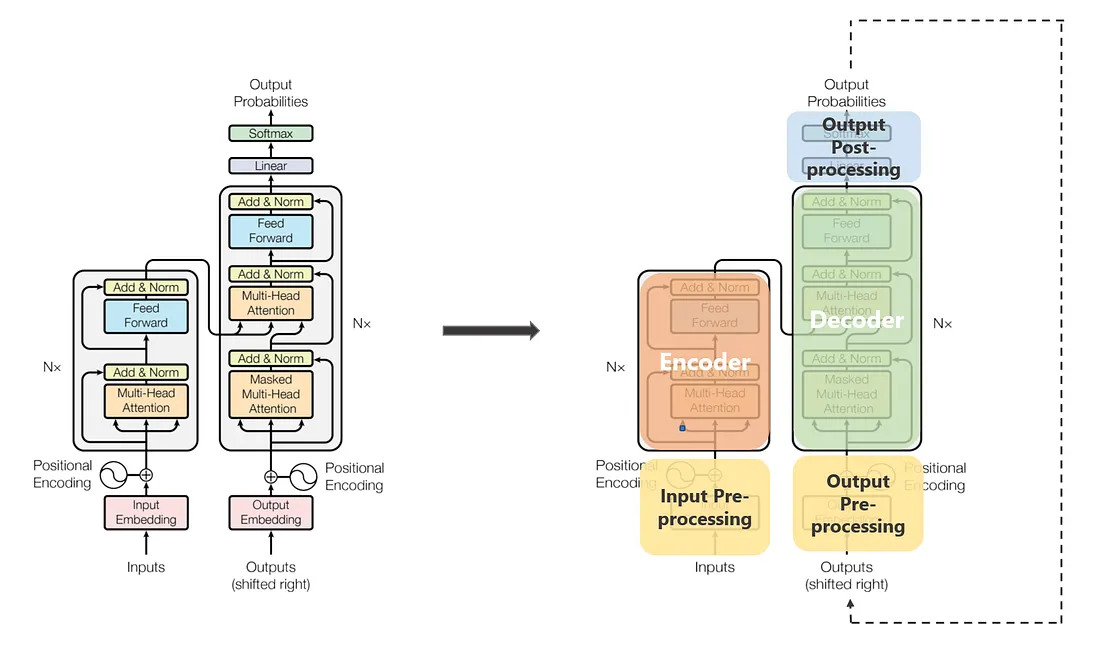
\includegraphics[width=\linewidth, height=0.72\textheight, keepaspectratio]{figures/transformers_view.png}
% \end{center}

% \column{0.47\textwidth}

% \vspace{4pt}

% \onslide<2->{
% \begin{block}{Key components}
% \begin{itemize}
%   \item \textbf{Token + positional embeddings}: words and positions $\to$ vectors
%   \item \textbf{Multi-head self-attention}: context-sensitive mixing across all positions
%   \item \textbf{Feed-forward sub-layer}: per-position nonlinear transform
%   \item \textbf{Residual connections} + \textbf{layer norm}: depth and stability
% \end{itemize}
% \end{block}
% }

% \onslide<3->{
% \vspace{6pt}
% For language modeling, stack $N$ blocks with a \textbf{causal mask} so each position attends only to itself and the past.
% }

% \end{columns}

% \end{frame}

% ---------------------------------------------------------------------------
\begin{frame}{The Attention Mechanism}

\begin{center}
\only<1>{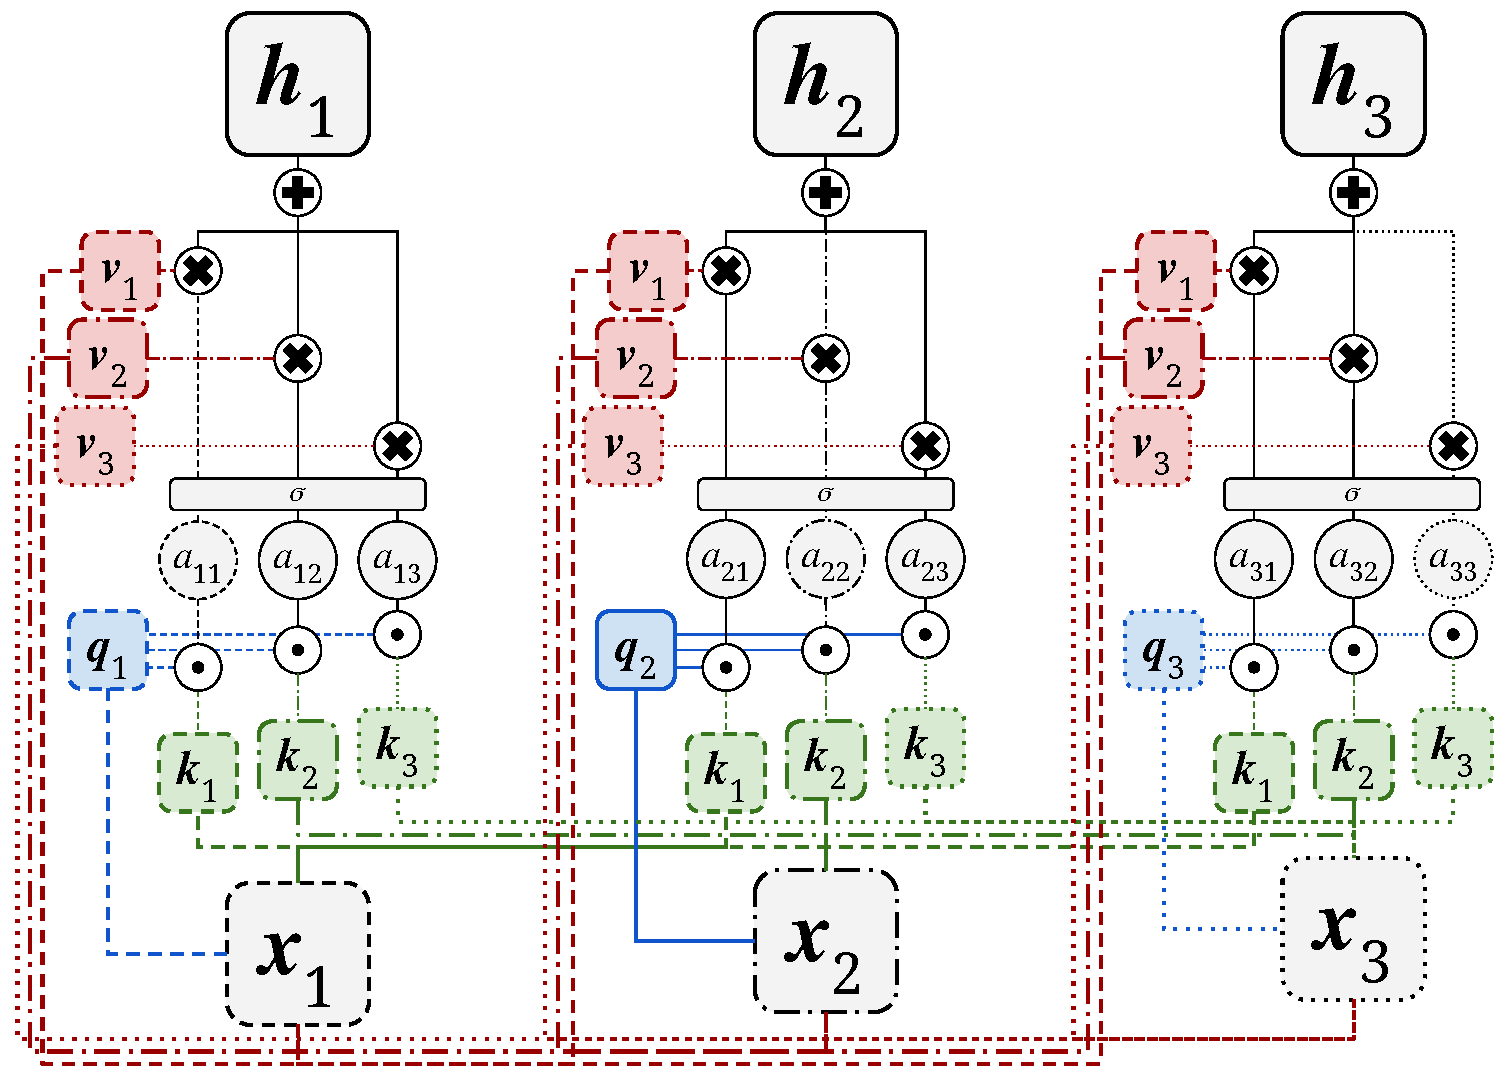
\includegraphics[height=0.9\textheight, keepaspectratio]{figures/Bidirectional Attention.pdf}}
\only<2>{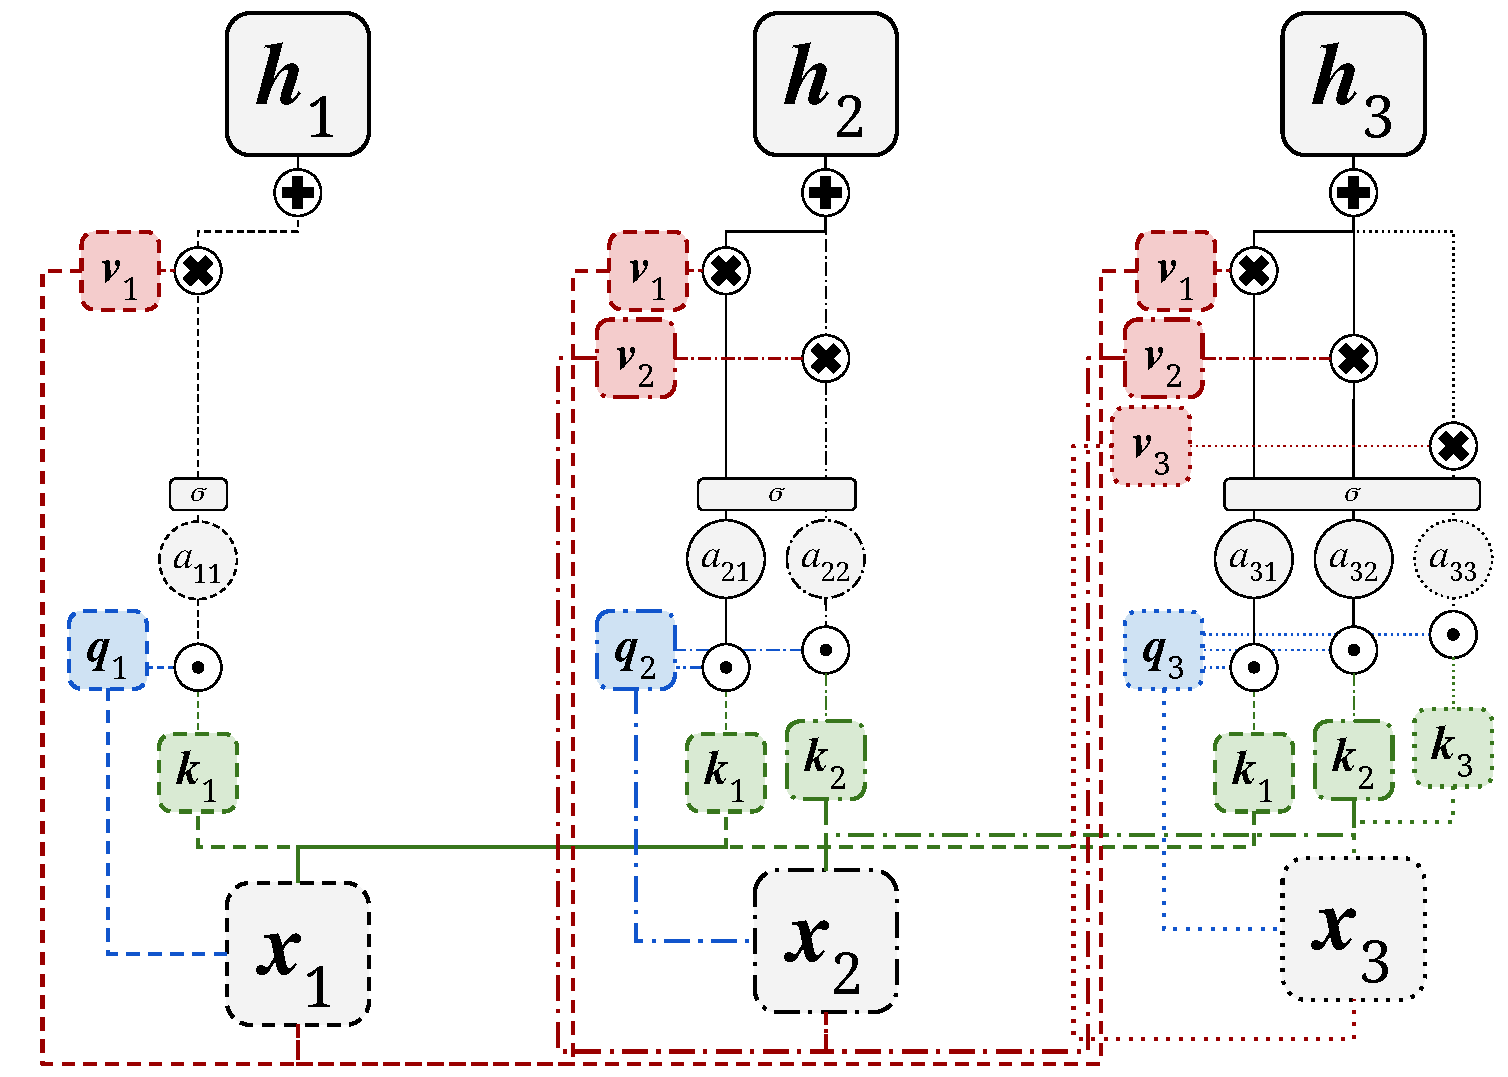
\includegraphics[height=0.9\textheight, keepaspectratio]{figures/Causal Attention.pdf}}
\end{center}

\end{frame}

% ---------------------------------------------------------------------------
% \begin{frame}{Causal vs.\ Bidirectional Attention}

% \begin{columns}[T]
% \column{0.49\textwidth}
% \begin{center}
% \textbf{Causal (GPT family)}\\[4pt]
% 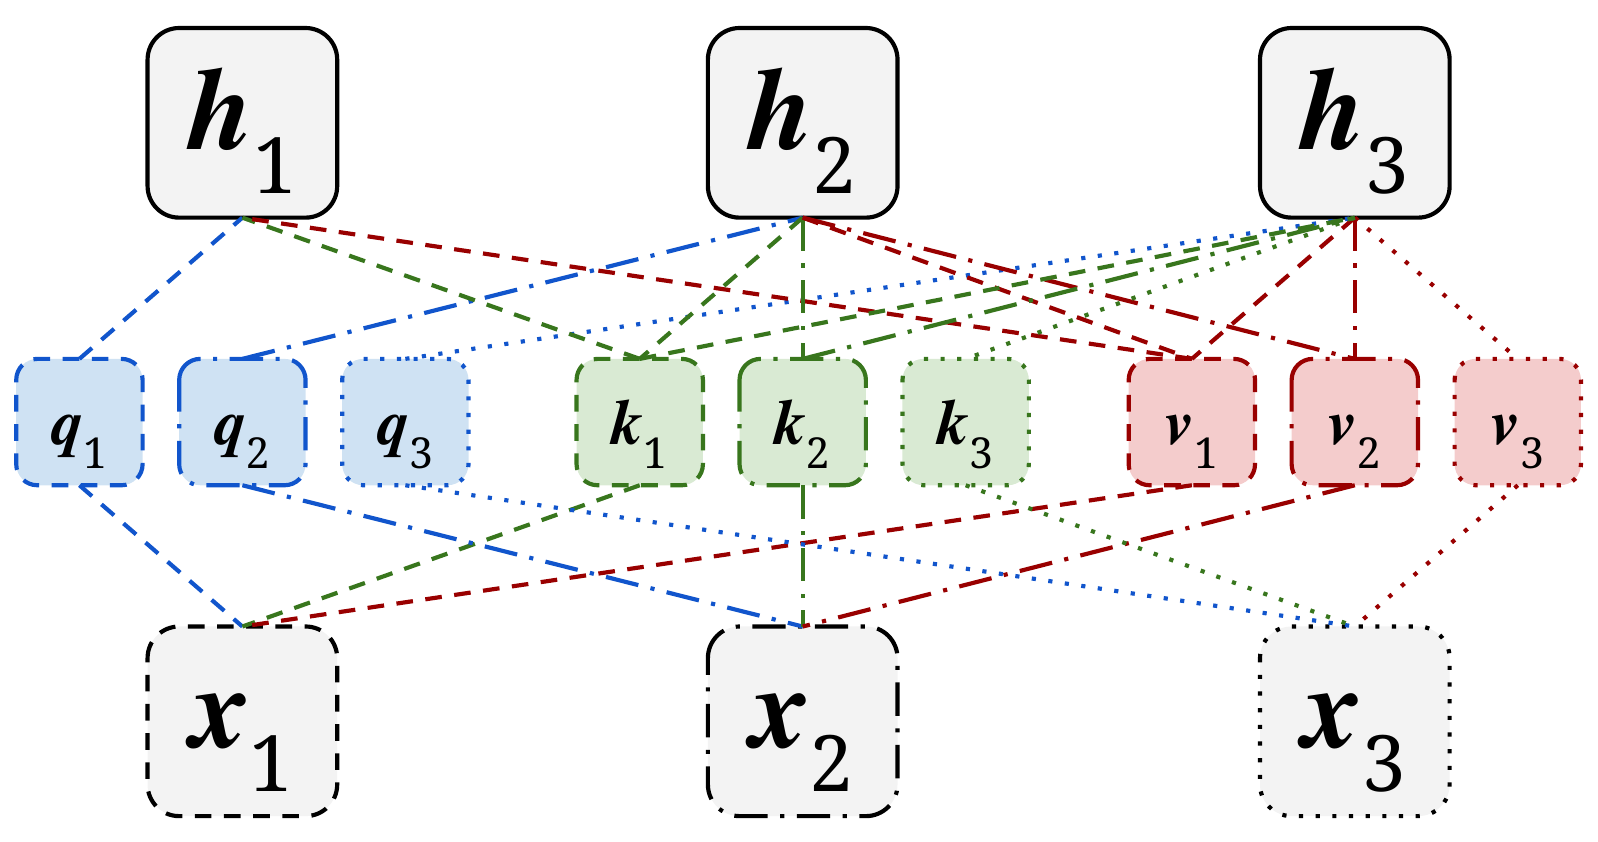
\includegraphics[width=\linewidth, height=0.62\textheight, keepaspectratio]{figures/causal_flow_only.png}
% \end{center}

% \column{0.49\textwidth}
% \begin{center}
% \textbf{Bidirectional (BERT family)}\\[4pt]
% 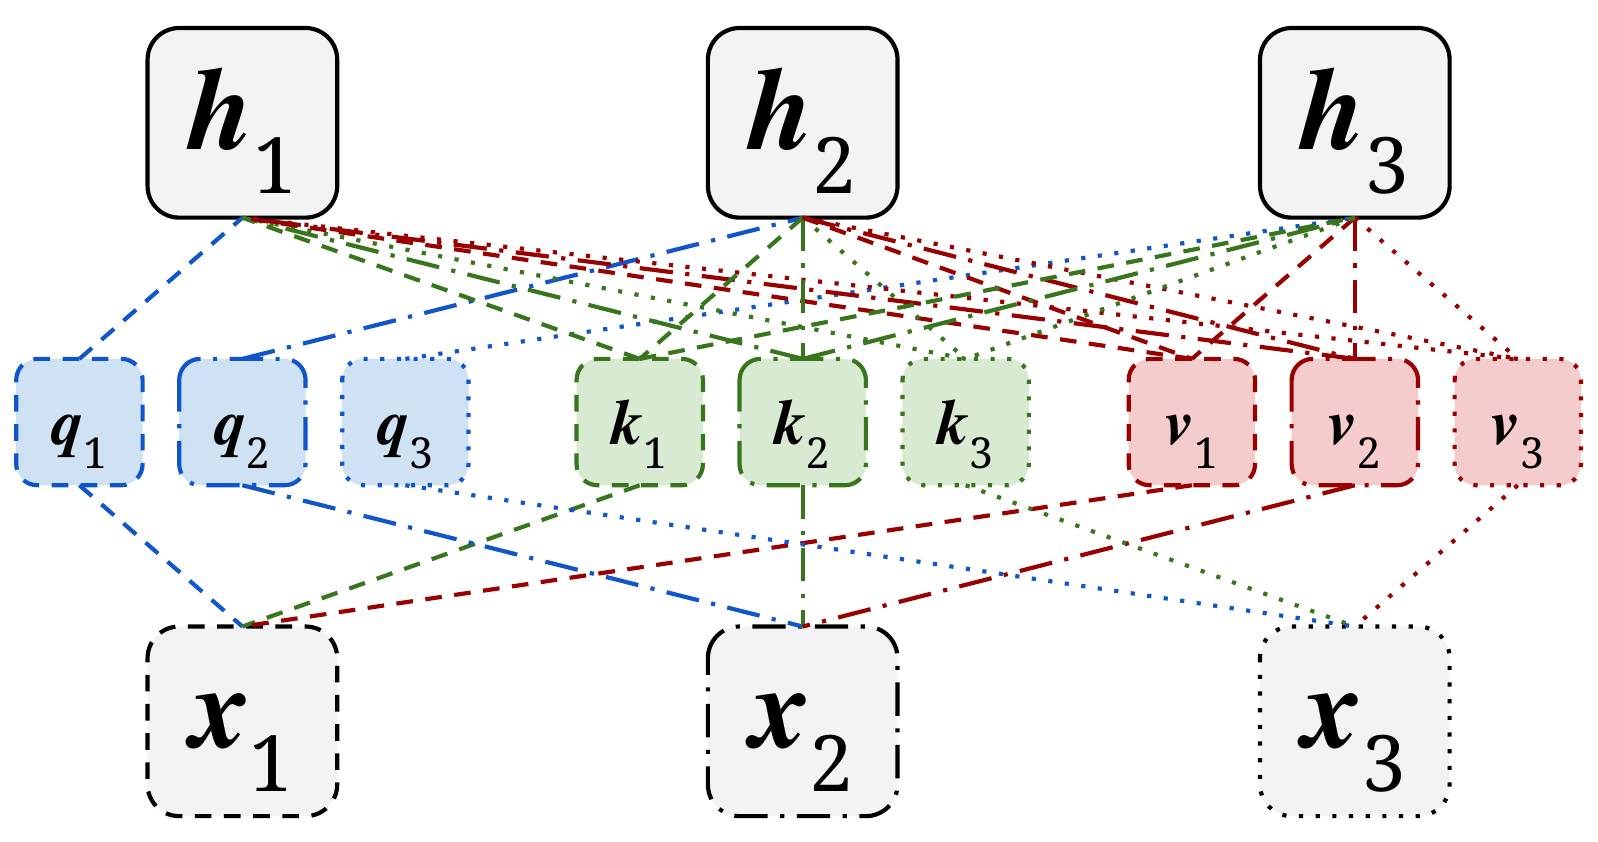
\includegraphics[width=\linewidth, height=0.62\textheight, keepaspectratio]{figures/bidir_flow_only.png}
% \end{center}
% \end{columns}

% \vspace{4pt}
% \begin{center}
% \small Each token $\mathbf{x}_i$ produces $\mathbf{q}_i$, $\mathbf{k}_i$, $\mathbf{v}_i$.
% Arrows show which keys each query can attend to.
% \textbf{Causal}: future tokens masked out (language modeling).
% \textbf{Bidirectional}: full context (classification, retrieval).
% \end{center}

% \end{frame}

% ---------------------------------------------------------------------------
\begin{frame}{§5 Notebook: BioMedLM Attention on a Clinical Sentence}

\begin{center}
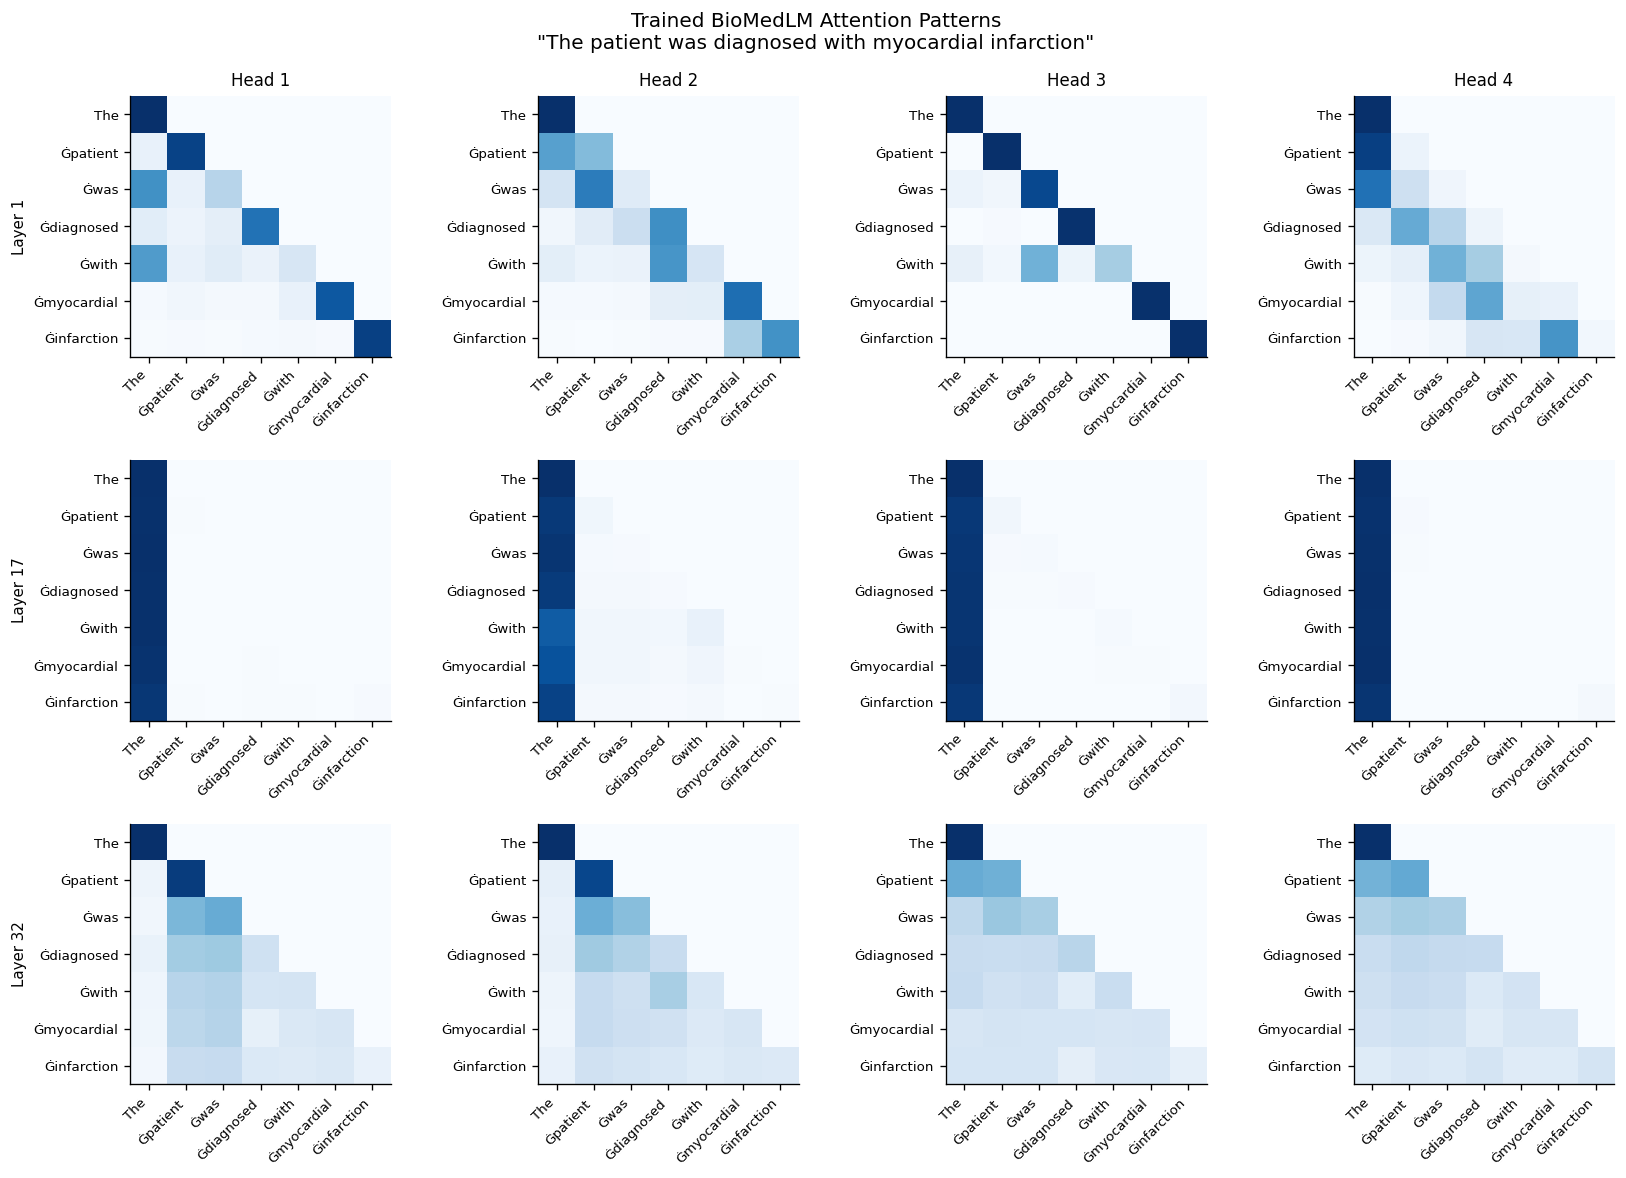
\includegraphics[width=0.96\textwidth, height=0.62\textheight, keepaspectratio]{figures/nb_biomedlm_attention.png}
\end{center}

\begin{center}
\small\textit{12 heads (3 layers) on ``The patient was diagnosed with myocardial infarction.'' Early: local/positional. Later: semantic --- does any head link ``infarction'' back to ``myocardial''?}
\end{center}

\end{frame}

% ---------------------------------------------------------------------------
\begin{frame}{Go Deeper: Interactive Resources}

\begin{block}{Transformer Explainer \hfill \url{https://poloclub.github.io/transformer-explainer/}}
\vspace{3pt}
Live in-browser GPT-2 visualization --- step through tokenization, embeddings, every attention head, and next-token prediction in real time. Great to open in class.
\end{block}

\vspace{6pt}

\begin{block}{The Illustrated Transformer}
\vspace{3pt}
Jay Alammar's canonical visual walkthrough. Best introduction to attention; used at Stanford, MIT, CMU, Princeton.\\[3pt]
\url{https://jalammar.github.io/illustrated-transformer/}
\end{block}

\vspace{10pt}
\begin{center}
\textit{Suggested: read Alammar, then open the Explainer with a prompt of your choosing,\\ then revisit the math in the slides and Notebook \S3.}
\end{center}

\end{frame}

% ---------------------------------------------------------------------------
\begin{frame}{Three Intuitions for Attention}

\begin{columns}[T]
\column{0.32\textwidth}
\onslide<1->{
\begin{block}{1.\ Probabilistic expectation}
\vspace{4pt}
\[
\text{out}_t = \mathbb{E}_{s \sim \alpha_{t\cdot}}\bigl[\mathbf{v}_s\bigr]
\]
$\alpha_{ts}$ is a \textbf{distribution} over positions. Output is the expected value vector under that distribution.
\end{block}
}

\column{0.32\textwidth}
\onslide<2->{
\begin{block}{2.\ Soft retrieval}
\vspace{4pt}
\textbf{Q}ueries ask a question.\\
\textbf{K}eys are index entries.\\
\textbf{V}alues hold the content.

\vspace{4pt}
Like a database lookup --- but \textbf{differentiable}: gradients flow through the retrieval.
\end{block}
}

\column{0.32\textwidth}
\onslide<3->{
\begin{block}{3.\ Token self-revision}
\vspace{4pt}
Each token has a current representation. It \emph{exposes} that to the rest of the sequence, then \emph{looks around} at everyone else to decide: given what I see, how should I revise my own representation for the next layer?
\end{block}
}
\end{columns}

\vspace{6pt}
\onslide<4->{
\begin{columns}[b]
\column{0.55\textwidth}
\begin{center}
$\alpha_{ts} = \text{softmax}\!\left(\dfrac{\mathbf{q}_t^\top \mathbf{k}_s}{\sqrt{d_k}}\right)$\\[4pt]
\small (scaling by $\sqrt{d_k}$ prevents softmax saturation)
\end{center}

% \column{0.42\textwidth}
% \begin{center}
% 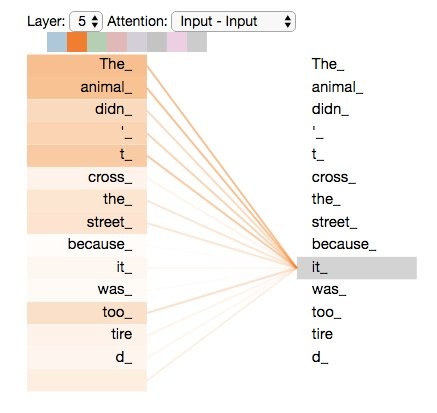
\includegraphics[width=\linewidth, height=0.30\textheight, keepaspectratio]{figures/self_attn_viz.png}\\[2pt]
% \small\textit{``it'' attends to ``animal'' --- token self-revision in action}
% \end{center}
\end{columns}
}

\end{frame}

% ---------------------------------------------------------------------------
\begin{frame}{Inside a Transformer Block}

\onslide<1->{
Each block applies two sub-layers with \textbf{residual connections}:
}

\vspace{8pt}
\onslide<2->{
\[
\mathbf{x}' = \mathbf{x} + \text{MultiHeadAttention}\!\bigl(\text{LayerNorm}(\mathbf{x})\bigr)
\]
}
\onslide<3->{
\[
\mathbf{x}'' = \mathbf{x}' + \text{FeedForward}\!\bigl(\text{LayerNorm}(\mathbf{x}')\bigr)
\]
}

\vspace{8pt}

\onslide<4->{
\begin{block}{Why residuals?}
Each block \textbf{adds} a correction to a running representation --- it never replaces it. This lets gradients flow cleanly through 100+ layers and prevents vanishing gradient problems.
\end{block}
}

\vspace{8pt}

\onslide<5->{
\begin{block}{Why layer norm?}
Normalizes activations before each sub-layer (Pre-LN variant). Stabilizes magnitudes during training and reduces sensitivity to learning rate choice.
\end{block}
}

\onslide<5->{
\vspace{6pt}
\notebookcallout{3}{Implement a Transformer block from scratch in PyTorch. Verify causal masking. Visualize attention weights on a sample sentence.}
}

\end{frame}

% ---------------------------------------------------------------------------
\begin{frame}{Positional Encoding: Teaching Order Without Recurrence}

\onslide<1->{
\begin{alertblock}{The problem}
Attention is \textbf{permutation-invariant}: without extra information, \textit{``dog bites man''} and \textit{``man bites dog''} are indistinguishable.
\end{alertblock}
}

\vspace{10pt}

\onslide<2->{
\begin{block}{Sinusoidal encoding (Vaswani et al., 2017)}
\[
\text{PE}_{t,2i} = \sin\!\left(\frac{t}{10000^{2i/d}}\right)
\]
A fixed vector added to each token embedding. Different frequencies encode position at different scales --- nearby tokens share low-frequency components; exact positions differ at high frequencies.
\end{block}
}

\end{frame}

% ---------------------------------------------------------------------------
\begin{frame}{Modern Positional Encoding Schemes}

\begin{block}{Learned absolute PE \hfill (GPT-2, BERT)}
\vspace{4pt}
One trainable embedding per position. Simple, effective within training length, but does not extrapolate beyond it.
\end{block}

\vspace{8pt}

\onslide<2->{
\begin{block}{RoPE --- Rotary Position Embedding \hfill (LLaMA, GPT-NeoX)}
\vspace{4pt}
Encodes \emph{relative} position by rotating Q and K vectors before the dot product. Better length generalization than absolute PE; now the dominant approach.
\end{block}
}

\vspace{8pt}

\onslide<3->{
\begin{exampleblock}{Key limitation}
Position is an \textbf{indirect} inductive bias regardless of scheme --- the model must \emph{learn} to use it. Unlike RNNs where order is architecturally enforced, this creates measurable degradation on long contexts (revisited in Open Challenges).
\end{exampleblock}
}

\end{frame}

% ---------------------------------------------------------------------------
\begin{frame}{What Made Transformers Actually Work}

\begin{columns}[T]
\column{0.48\textwidth}
\onslide<1->{
\begin{block}{Architectural}
\begin{itemize}
  \item Scaled dot-product attention ($\div\sqrt{d_k}$)
  \item Multi-head attention (parallel specialization)
  \item Residual connections (deep training)
  \item Layer normalization (stability)
  \item Large FFN sub-layer ($4\times$ hidden dim)
  \item Byte-pair encoding (open vocabulary)
\end{itemize}
\end{block}
}

\column{0.48\textwidth}
\onslide<2->{
\begin{block}{Training and alignment}
\begin{itemize}
  \item \textbf{Scale}: trillions of tokens, billions of params
  \item \textbf{Instruction fine-tuning}: task and format following
  \item \textbf{RLHF}: human preferences $\to$ reward model $\to$ PPO
  \item \textbf{DPO}: direct preference optimization
  \item \textbf{Constitutional AI}: self-critique loop
\end{itemize}
\end{block}
}
\end{columns}

\onslide<3->{
\vspace{6pt}
\begin{center}
\textit{No single ingredient is magic. The combination --- at scale --- produced emergent capability.}
\end{center}
}

\end{frame}

% ---------------------------------------------------------------------------
\begin{frame}{Mathematical Challenge: Quadratic Attention Cost}

\onslide<1->{
Computing attention requires \textbf{all} $T \times T$ pairwise scores:
\[
\text{Attention}(\mathbf{Q}, \mathbf{K}, \mathbf{V})
= \text{softmax}\!\left(\frac{\mathbf{Q}\mathbf{K}^\top}{\sqrt{d_k}}\right)\mathbf{V}
\]
\textbf{Complexity:} $\mathcal{O}(T^2 d)$ time and $\mathcal{O}(T^2)$ memory.
}

\vspace{4pt}

\begin{columns}[T]
\column{0.45\textwidth}
\onslide<2->{
\begin{alertblock}{Practical impact}
\begin{itemize}
  \item $T = 1{,}024$: $\sim$1M attention pairs
  \item $T = 8{,}192$: $\sim$67M pairs
  \item $T = 128{,}000$: $\sim$16B pairs
\end{itemize}
Context window = hard engineering constraint.
\end{alertblock}
}

\column{0.52\textwidth}
\onslide<3->{
\begin{block}{Active solutions}
\begin{itemize}
  \item \textbf{FlashAttention}: I/O-aware; same $O(T^2)$ ops, 2--4$\times$ faster in practice.
  \item \textbf{Sliding window}: Longformer, BigBird --- local $\mathcal{O}(T)$ attention.
  \item \textbf{State space models}: Mamba, S4 --- $\mathcal{O}(T)$ with recurrent structure.
\end{itemize}
\end{block}
}
\end{columns}

\onslide<3->{
\vspace{2pt}
\notebookcallout{3}{Plot attention memory cost vs.\ $T$. Overlay GPU VRAM limits to see why long-context is hard.}
}

\end{frame}

% ---------------------------------------------------------------------------
\begin{frame}{Challenge: Exact Decoding is Intractable}

\onslide<1->{
Greedy decoding: at each step pick $\arg\max_v P(w_{t+1}=v\mid\text{context})$.

\vspace{6pt}
But the \textbf{globally most-likely sequence} is not the product of greedy local choices.
}

\vspace{8pt}

\begin{columns}[T]
\column{0.48\textwidth}
\onslide<2->{
\begin{block}{Decoding strategies}
\begin{itemize}
  \item \textbf{Beam search}: keep top-$k$ sequences; better quality
  \item \textbf{Temperature sampling}: rescale logits; diverse, creative
  \item \textbf{Nucleus (top-$p$)}: sample from smallest set covering probability $p$
\end{itemize}
\end{block}
}

\column{0.48\textwidth}
\onslide<3->{
\begin{alertblock}{Do we want the ``most likely''?}
``Does this patient have rare cancer X?'' --- the maximally likely answer is almost always \emph{No}, even when the patient is far more likely than baseline to have it.\\
Maximum likelihood $\neq$ calibrated inference.
\end{alertblock}
}
\end{columns}

\onslide<3->{
\vspace{6pt}
\notebookcallout{4}{Compare greedy, temperature, and nucleus sampling on a clinical prompt. Observe output variance.}
}

\end{frame}

% ---------------------------------------------------------------------------
\begin{frame}{§4 Notebook: How Temperature Reshapes the Distribution}

\begin{center}
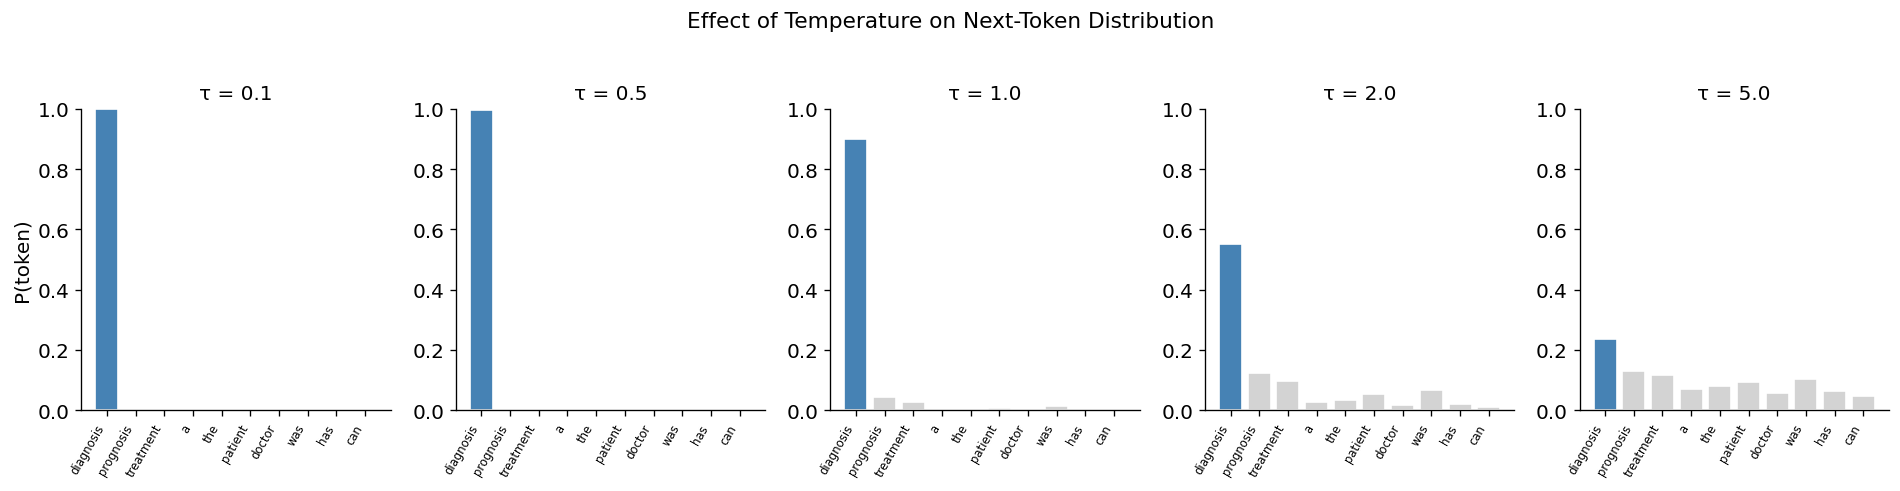
\includegraphics[width=0.95\textwidth]{figures/nb_temperature.png}
\end{center}

\vspace{2pt}
\begin{center}
\textit{Low temperature ($\tau \to 0$) collapses mass onto the mode --- greedy decoding. High temperature flattens the distribution, increasing diversity at the cost of coherence.}
\end{center}

\end{frame}

% ---------------------------------------------------------------------------
\begin{frame}{§5 Notebook: Five Strategies, Four Diagnoses}

\onslide<1->{
Prompt: \textit{``The patient presents with acute chest pain and shortness of breath. The most likely diagnosis is''}
}

\vspace{6pt}

\begin{columns}[T]
\column{0.50\textwidth}
\onslide<2->{
\begin{exampleblock}{Greedy}
\vspace{2pt}
``\dots\ \textbf{pulmonary embolism}.'' (then generates MCQ-style artifacts from PubMed training data)
\end{exampleblock}
}
\onslide<3->{
\begin{exampleblock}{Beam search ($k=4$)}
\vspace{2pt}
``\dots\ \textbf{acute coronary syndrome (ACS)}.''
\end{exampleblock}
}
\onslide<4->{
\begin{exampleblock}{Temperature $\tau=0.7$}
\vspace{2pt}
``\dots\ \textbf{pulmonary embolism}. Her history includes hypertension, hypercholesterolemia, and remote DVT\dots'' \good{(most fluent)}
\end{exampleblock}
}

\column{0.47\textwidth}
\onslide<5->{
\begin{alertblock}{Nucleus $p=0.9$}
\vspace{2pt}
``\dots\ \textbf{pericarditis}.''
\end{alertblock}
}
\onslide<5->{
\begin{alertblock}{Top-$k$ ($k=50$)}
\vspace{2pt}
``\dots\ \textbf{coronary artery disease with acute ischemia}.''
\end{alertblock}
}
\onslide<6->{
\begin{block}{}
Same model, same prompt, five different answers. In clinical deployment: which do you report? How do you know which is right?
\end{block}
}
\end{columns}

\end{frame}

% ===========================================================================
\section{The LLM Ecosystem}
% ===========================================================================

% ---------------------------------------------------------------------------
\begin{frame}{The LLM Landscape}

\begin{columns}[T]
\column{0.32\textwidth}
\onslide<1->{
\begin{block}{Proprietary APIs}
\begin{itemize}
  \item GPT (OpenAI)
  \item Claude (Anthropic)
  \item Gemini (Google)
\end{itemize}
\vspace{4pt}
Easy to use; \bad{data sent to third-party servers}.
\end{block}
}

\column{0.32\textwidth}
\onslide<2->{
\begin{block}{Open weights}
\begin{itemize}
  \item LLaMA (Meta)
  \item Mistral / Mixtral
  \item Phi-3 (Microsoft)
  \item Qwen, Gemma, \dots
\end{itemize}
\vspace{4pt}
Downloadable. Customizable. Local deployment possible.
\end{block}
}

\column{0.32\textwidth}
\onslide<3->{
\begin{alertblock}{Health AI constraint}
For clinical data (HIPAA), \textbf{local deployment} of open-weight models may be required. Proprietary APIs send PHI to external servers.
\end{alertblock}
\vspace{4pt}
\begin{block}{Infrastructure}
HuggingFace Hub, Ollama, vLLM, SGLang
\end{block}
}
\end{columns}

\end{frame}

% ---------------------------------------------------------------------------
\begin{frame}{HuggingFace: The GitHub of AI Models}

\begin{columns}[T]
\column{0.48\textwidth}
\onslide<1->{
\begin{block}{What it provides}
\begin{itemize}
  \item \textbf{Model Hub}: 500K+ pre-trained models
  \item \textbf{Datasets}: 100K+ curated datasets
  \item \textbf{Transformers}: one unified API for all architectures
  \item \textbf{PEFT}: LoRA, prefix tuning, adapters
  \item \textbf{Accelerate}: multi-GPU / distributed training
\end{itemize}
\end{block}
}

\column{0.48\textwidth}
\onslide<2->{
\begin{exampleblock}{Two lines to a language model}
\vspace{4pt}
\texttt{\small from transformers import pipeline}\\[2pt]
\texttt{\small gen = pipeline(}\\
\texttt{\small \quad "text-generation", model="gpt2")}\\[2pt]
\texttt{\small gen("The patient presents",}\\
\texttt{\small \quad max\_new\_tokens=40)}
\vspace{4pt}
\end{exampleblock}
}
\end{columns}

\vspace{6pt}
\onslide<2->{
\notebookcallout{5}{Load GPT-2 via HuggingFace. Inspect medical tokenization. Generate text. Visualize trained attention. Compute perplexity.}
}

\end{frame}

% ---------------------------------------------------------------------------
\begin{frame}{Running LLMs Locally: Quantization and LoRA}

\begin{columns}[T]
\column{0.50\textwidth}
\onslide<1->{
\begin{block}{The memory problem}
LLaMA 3 70B at full precision: \textbf{140 GB}.\\
An A100 GPU: 80 GB. \quad RTX 4090: 24 GB.

\vspace{6pt}
\textbf{Quantization} compresses weights:
\begin{itemize}
  \item fp16 / bf16: $\sim$$2\times$ compression, tiny quality loss
  \item INT8: $\sim$$4\times$ compression (bitsandbytes)
  \item GGUF 4-bit (Ollama): 70B fits on a laptop
\end{itemize}
\end{block}
}

\column{0.47\textwidth}
\onslide<2->{
\begin{block}{LoRA: fine-tune without full weights}
\vspace{2pt}
Freeze $\mathbf{W}_0 \in \mathbb{R}^{d \times d}$. Add a low-rank correction $\mathbf{AB}$:

\vspace{4pt}
\begin{center}
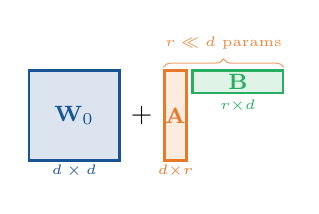
\begin{tikzpicture}[scale=0.52]
  % Big square W0
  \draw[ColumbiaBlue, fill=ColumbiaBlue!15, line width=1pt] (0,0) rectangle (2.2,2.2);
  \node[ColumbiaBlue, font=\footnotesize\bfseries] at (1.1,1.1) {$\mathbf{W}_0$};
  \node[font=\tiny, ColumbiaBlue] at (1.1,-0.25) {$d \times d$};
  % plus
  \node[font=\normalsize] at (2.75,1.1) {$+$};
  % A (tall thin)
  \draw[AccentOrange, fill=AccentOrange!15, line width=1pt] (3.3,0) rectangle (3.85,2.2);
  \node[AccentOrange, font=\footnotesize\bfseries] at (3.575,1.1) {$\mathbf{A}$};
  \node[font=\tiny, AccentOrange] at (3.575,-0.25) {$d{\times}r$};
  % B (short wide)
  \draw[AccentGreen, fill=AccentGreen!15, line width=1pt] (4.0,1.65) rectangle (6.2,2.2);
  \node[AccentGreen, font=\footnotesize\bfseries] at (5.1,1.925) {$\mathbf{B}$};
  \node[font=\tiny, AccentGreen] at (5.1,1.35) {$r{\times}d$};
  % brace
  \draw[decorate, decoration={brace,amplitude=3pt}, AccentOrange!70] (3.28,2.28) -- (6.22,2.28)
    node[midway, above=3pt, font=\tiny, AccentOrange!90] {$r \ll d$ params};
\end{tikzpicture}
\end{center}

\vspace{2pt}
$r{=}8$, $d{=}4096$: $\mathbf{AB}$ has $2{\times}8{\times}4096 \approx 65$K params vs.\ $4096^2 \approx 17$M --- $>$99\% savings.
\end{block}
}
\end{columns}

\end{frame}

% ===========================================================================
\section{Open Challenges}
% ===========================================================================

% ---------------------------------------------------------------------------
\begin{frame}{Challenge: Hallucination}

\onslide<1->{
\begin{alertblock}{What is hallucination?}
LLMs generate confident, fluent, plausible-sounding text that is \textbf{factually wrong}.

\vspace{4pt}
\textbf{Why?} The model optimizes for likely text, not true text:
\[
\arg\max P(\mathbf{w}_{1:T}) \;\neq\; \arg\max P(\mathbf{w}_{1:T} \mid \text{w is true})
\]
There is no explicit truth signal in next-token prediction training.
\end{alertblock}
}

\vspace{6pt}
\begin{columns}[T]
\column{0.48\textwidth}
\onslide<2->{
\begin{block}{Health AI consequences}
\begin{itemize}
  \item Fabricated drug interactions
  \item Incorrect dosages, stated confidently
  \item Non-existent guidelines cited
  \item False patient summaries
\end{itemize}
\end{block}
}

\column{0.48\textwidth}
\onslide<3->{
\begin{exampleblock}{Mitigations}
\begin{itemize}
  \item \textbf{RAG}: ground outputs in retrieved facts
  \item Forced source attribution
  \item Train on ``I don't know''
  \item Human-in-the-loop verification
\end{itemize}
\end{exampleblock}
}
\end{columns}

\end{frame}

% ---------------------------------------------------------------------------
\begin{frame}{Reasoning, Scale, and the Active Frontier}

\begin{columns}[T]
\column{0.48\textwidth}
\onslide<1->{
\begin{block}{Chain of Thought (Wei et al., 2022)}
Prompting models to emit \textbf{intermediate steps} dramatically improves multi-step reasoning:
\[
Q \to \text{step}_1 \to \cdots \to \text{step}_k \to A
\]
Extensions: Tree of Thought, Graph of Thought, self-consistency.
\end{block}
}
\onslide<2->{
\begin{block}{Test-time compute}
OpenAI o1, DeepSeek-R1: scale reasoning at \textbf{inference} rather than only at training time. Models ``think longer'' on hard problems.
\end{block}
}

\column{0.48\textwidth}
\onslide<3->{
\begin{block}{Architectural frontier}
\begin{itemize}
  \item \textbf{MoE} (Mixture of Experts): sparse activation, only a fraction of parameters fire per token (Mixtral, GPT-4, DeepSeek-V3)
  \item \textbf{SSMs} (Mamba, RWKV): $\mathcal{O}(T)$ alternatives to attention
  \item \textbf{RAG}: retrieve relevant docs at inference time
  \item \textbf{Agentic LLMs}: tool use, code execution, multi-agent pipelines
\end{itemize}
\end{block}
}
\end{columns}

\end{frame}

% ---------------------------------------------------------------------------
\begin{frame}{We Built the Chinese Room}

\begin{columns}[T]
\column{0.52\textwidth}

\onslide<1->{
\begin{block}{What we built}
\begin{itemize}
  \item<2-> A conditional probability estimator over token sequences
  \item<3-> Trained on the combinatorially vast space of human-written text
  \item<4-> Using attention to dynamically route context across any distance
  \item<5-> With \emph{no} explicit world model, no causal structure, no truth signal
\end{itemize}
\vspace{4pt}
\onslide<5->{ChatGPT, Claude, Gemini: billions of parameters, no grounding.\\
Searle's thought experiment \textbf{became a product}.}
\end{block}
}

\column{0.45\textwidth}

\onslide<6->{
\begin{alertblock}{And it works.}
\vspace{4pt}
It passes the bar exam.\\
It diagnoses rare diseases from notes.\\
It writes code, poetry, legal briefs.

\vspace{6pt}
\textbf{Does it understand any of it?}

\vspace{6pt}
Searle said: impossible.\\
We built it anyway.\\
The question is now empirical --- and open.
\end{alertblock}
}

\end{columns}

\onslide<7->{
\vspace{6pt}
\begin{center}
\large\textit{The math is clear. The implications are not.}\\[4pt]
\textcolor{AccentOrange}{\ding{118}}\; We are now in the post-paradox world. How we answer that question shapes how we deploy, trust, and regulate LLMs in healthcare.
\end{center}
}

\end{frame}

% ---------------------------------------------------------------------------
\begin{frame}{What Does ``Understand'' Mean?}

\begin{center}
{\large Searle's argument turns on a word we haven't defined.}
\end{center}

\vspace{4pt}

\begin{columns}[T]
\column{0.48\textwidth}
\onslide<2->{
\begin{block}{Behavioral criterion}
If a system responds to every situation the way an understander would, what more could ``understanding'' mean?

\vspace{2pt}
\textit{``If it walks like a duck\dots''}
\end{block}
}

\column{0.48\textwidth}
\onslide<3->{
\begin{alertblock}{Intentional criterion}
Understanding requires \emph{aboutness}: mental states genuinely about things in the world. Syntax can never produce semantics.
\end{alertblock}
}
\end{columns}

\vspace{4pt}
\onslide<4->{
\begin{exampleblock}{The empirical question}
Do LLMs generalize, reason, and fail in the ways a \emph{understander} would --- or a \emph{very good pattern-matcher} would? \onslide<5->{\textbf{And does it matter?}}
\end{exampleblock}
}

\end{frame}

% ---------------------------------------------------------------------------
\begin{frame}{Summary}

\begin{columns}[T]
\column{0.52\textwidth}
\begin{itemize}
  \item<1-> \textbf{Language modeling}: next-word prediction $\equiv$ sequence probability $\equiv$ generation.
  \item<2-> \textbf{Why it's hard}: context space exceeds atoms in the universe; lookup fails; n-grams miss long dependencies.
  \item<3-> \textbf{Transformers}: attention gives variable-length, long-range, parallel context --- at $\mathcal{O}(T^2)$ cost.
  \item<4-> \textbf{Ecosystem}: HuggingFace, quantization, LoRA enable local clinical deployment.
  \item<5-> \textbf{Open}: hallucination, decoding, position generalization, reasoning, agents.
\end{itemize}

\column{0.45\textwidth}
\onslide<6->{
\begin{exampleblock}{Companion notebook}
\vspace{2pt}
\begin{tabular}{@{}ll@{}}
\S1 & Context match statistics \\
\S2 & N-gram models \& generation \\
\S3 & Transformer from scratch \\
\S4 & Decoding strategies \\
\S5 & HuggingFace inference \\
\end{tabular}
\end{exampleblock}
}
\vspace{4pt}
\onslide<6->{
\begin{block}{Key readings}
\scriptsize
Vaswani et al.\ (2017) ``Attention is All You Need''\\
Brown et al.\ (2020) ``GPT-3''\\
Liu et al.\ (2023) ``Lost in the Middle''\\
Hu et al.\ (2021) ``LoRA''
\end{block}
}
\end{columns}

\end{frame}

% ===========================================================================
\appendix

% ---------------------------------------------------------------------------
{
\setbeamercolor{background canvas}{bg=black}
\begin{frame}[plain]{}
\end{frame}
}

% ---------------------------------------------------------------------------
\begin{frame}{The Historical Path: RNNs to Transformers}

\begin{exampleblock}{Why ``decoder-only''?}
The original Transformer (Vaswani 2017) had an \emph{encoder} (reads the full source) and a \emph{decoder} (generates the target). GPT-family models dropped the encoder --- the decoder alone, trained on next-token prediction, turns out to be enough for almost everything.
\end{exampleblock}

\vspace{8pt}
\begin{block}{RNNs and LSTMs (1990s--2017)}
\vspace{4pt}
Handle variable-length sequences naturally. But computation is \textbf{sequential} --- each step depends on the last --- making parallelization impossible. Gradients also \textbf{vanish} over long distances, limiting effective context.
\end{block}

\vspace{10pt}

\begin{exampleblock}{Transformers (Vaswani et al., 2017)}
\vspace{4pt}
\textbf{All-to-all attention}: every position can directly attend to every other in a single layer. Fully parallel. Scales to billions of parameters on modern hardware.

\vspace{6pt}
\begin{center}
\large\textit{``Attention is All You Need''}
\end{center}
\end{exampleblock}

\end{frame}

% ---------------------------------------------------------------------------
\begin{frame}{Further Reading: Bidirectional \& Encoder--Decoder Architectures}

\begin{block}{Self-study only --- not covered in lecture}
\vspace{2pt}
\begin{description}[leftmargin=2.0cm]
  \item[ELMo] Peters et al.\ (2018): contextualized embeddings from bidirectional LSTMs. First major contextual representation.
  \item[BERT] Devlin et al.\ (2018): bidirectional encoder, Masked Language Modeling + Next Sentence Prediction. Dominated benchmarks 2018--2021.
  \item[T5 / BART] Encoder--decoder: encoder reads full source, decoder generates target autoregressively. Used in translation and summarization.
  \item[GPT lineage] Decoder-only autoregressive models (GPT-1 through GPT-4o). Pre-trained on next-token prediction.
\end{description}
\vspace{4pt}
\textbf{Key reading:} Vaswani et al.\ (2017); Devlin et al.\ (2018) ``BERT''; Brown et al.\ (2020) ``GPT-3''
\end{block}

\end{frame}

% ---------------------------------------------------------------------------
\begin{frame}{§5 Notebook: How BioMedLM Tokenizes Medical Terms}

\onslide<1->{
Subword tokenization (BPE) splits on morpheme-like boundaries --- frequent roots become single tokens:
}

\vspace{4pt}

\begin{columns}[T]
\column{0.50\textwidth}
\onslide<2->{
\begin{exampleblock}{}
\texttt{"myocardial infarction"}\\
$\to$ \texttt{[`my', `ocardial', `infarction']}

\vspace{4pt}
\texttt{"electrocardiogram"}\\
$\to$ \texttt{[`electro', `cardi', `ogram']}

\vspace{4pt}
\texttt{"hypertension"}\\
$\to$ \texttt{[`hyper', `tension']}
\end{exampleblock}
}

\column{0.47\textwidth}
\onslide<2->{
\begin{exampleblock}{}
\texttt{"acetaminophen"}\\
$\to$ \texttt{[`acet', `aminophen']}

\vspace{4pt}
\texttt{"MIMIC-IV"}\\
$\to$ \texttt{[`MI', `MIC', `-', `IV']}

\vspace{4pt}
\texttt{"hemodynamically unstable"}\\
$\to$ \texttt{[`hem', `od', `ynamically', `unstable']}
\end{exampleblock}
}
\end{columns}

\vspace{4pt}
\onslide<3->{
\begin{block}{}
\small Roots like \texttt{cardio}, \texttt{hyper}, \texttt{electro} earn their own tokens. Rare terms fragment --- token count affects cost and performance.
\end{block}
}

\end{frame}

% ---------------------------------------------------------------------------
\begin{frame}{§5 Notebook: Perplexity --- What the Model Has Learned}

\onslide<1->{
\textbf{Perplexity} measures how surprised the model is by a sequence. Lower = more expected.
}

\vspace{8pt}

\onslide<2->{
\begin{center}
\begin{tabular}{@{}l r@{}}
\toprule
\textbf{Sentence (BioMedLM, trained on PubMed)} & \textbf{PPL} \\
\midrule
``The patient was admitted with ST-elevation myocardial\dots'' & \good{12.3} \\
``Troponin levels were elevated consistent with acute\dots''    & \good{15.9} \\
``The patient was started on aspirin, heparin\dots''            & \good{16.6} \\
\midrule
``The quick brown fox jumps over the lazy dog.''                & 107.8 \\
\midrule
Random gibberish tokens                                         & 326 \\
Scrambled clinical words (correct words, wrong order)           & \bad{11,043} \\
\bottomrule
\end{tabular}
\end{center}
}

\vspace{6pt}
\onslide<3->{
\begin{exampleblock}{What this tells us}
BioMedLM has internalized clinical language patterns so deeply that coherent biomedical prose is $\sim$9$\times$ less surprising than ordinary English --- and correct word order matters far more than correct vocabulary (scrambled $\approx$ 1000$\times$ worse than gibberish).
\end{exampleblock}
}

\end{frame}

% ---------------------------------------------------------------------------
\begin{frame}{Challenge: Indirect Position Dependence}

\onslide<1->{
\begin{alertblock}{Attention is order-blind without help}
Positional encoding is \textbf{learned}, not architecturally enforced. The model must figure out how to use it --- and doesn't always succeed.
\end{alertblock}
}

\vspace{8pt}

\begin{columns}[T]
\column{0.48\textwidth}
\onslide<2->{
\begin{block}{Length generalization}
Models often degrade on sequences \textbf{longer} than their training contexts, even with very long nominal context windows.
\end{block}
}

\column{0.48\textwidth}
\onslide<3->{
\begin{block}{Lost in the Middle}
Models attend much more strongly to the beginning and end of a long context than to the middle.

\vspace{4pt}
\textit{Liu et al., 2023 --- ``Lost in the Middle''}
\end{block}
}
\end{columns}

\vspace{8pt}
\onslide<4->{
\begin{exampleblock}{Why this matters clinically}
A long clinical note may have the most relevant finding buried in the middle --- exactly where the model is least likely to attend.
\end{exampleblock}
}

\end{frame}

% ===========================================================================
\end{document}
